% ============================================================================
% Dual Tetrad Gravity And The Field Origin
% Deriving Fundamental Equations With (3+1)^2 Topology
% Paper VII in the Distributed Field Processing Series
% ============================================================================
% Author: Stephen Nelson
% For arXiv/Physical Review submission
% ============================================================================

\documentclass[aps,prd,preprint,superscriptaddress,showpacs,preprintnumbers,amsmath,amssymb,nofootinbib]{revtex4-2}

% ============================================================================
% PACKAGES
% ============================================================================
\usepackage{graphicx}
\usepackage{amsmath,amssymb}
\usepackage{bm}
\usepackage{hyperref}
\usepackage{xcolor}
\definecolor{resultgreen}{HTML}{E1F2E2}
\usepackage{booktabs}
\usepackage{multirow}
\usepackage{float}
\usepackage{tikz}
\usetikzlibrary{arrows.meta,decorations.markings,calc}

% Hyperref setup
\hypersetup{
    colorlinks=true,
    linkcolor=blue!60!black,
    citecolor=blue!60!black,
    urlcolor=blue!60!black
}

% Paragraph formatting
\setlength{\parindent}{0pt}
\setlength{\parskip}{0.8ex plus 0.2ex minus 0.1ex}

% Equation spacing
\AtBeginDocument{%
  \abovedisplayskip=12pt plus 3pt minus 3pt
  \belowdisplayskip=12pt plus 3pt minus 3pt
  \abovedisplayshortskip=8pt plus 3pt minus 3pt
  \belowdisplayshortskip=8pt plus 3pt minus 3pt
}

% Box padding
\setlength{\fboxsep}{12pt}
\setlength{\fboxrule}{0.8pt}

% Abstract spacing (revtex4-2)
\makeatletter
\def\frontmatter@preabstractspace{0.75cm}
\makeatother

% ============================================================================
% DOCUMENT
% ============================================================================
\begin{document}
\raggedbottom

\vspace*{3cm}

% ----------------------------------------------------------------------------
% TITLE AND AUTHORS
% ----------------------------------------------------------------------------
\title{Dual Tetrad Gravity And The Field Origin\\
\large Deriving Fundamental Equations With $(3+1)^2$ Topology}

\author{Stephen Nelson}
\email[Contact author: ]{stephen@fielddynamics.org}
\affiliation{Independent Researcher\\ORCID: 0009-0008-6190-3269}

\date{February 2026}

% ----------------------------------------------------------------------------
% ABSTRACT
% ----------------------------------------------------------------------------
\begin{abstract}
The companion paper derived the gravitational constant $G$ from spacetime topology with 0.12\% accuracy and zero free parameters. This paper asks what else the same geometric structure determines.

The $(3+1)^2$ dual tetrad topology, two tetrahedra with opposite orientations coupled at a shared Field Origin, produces four quantitative results. (1)~$G$ from the coupling hierarchy $\alpha^{1+(3+1)+(3+1)^2}$, where changing the exponent by $\pm 1$ shifts the prediction by a factor of 137. (2)~The force hierarchy: gravity couples through 21 levels, electromagnetism through 1, giving $\alpha^{20} \approx 10^{-43}$. (3)~The dark matter correction factor $\mu(x) = x/(1+x)$, derived from detailed balance in field closure, with characteristic acceleration $a_0 = k^2 Gm_e/r_e^2$ (where $k = 4$ is the tetrahedral coupling number, $m_e$ the electron mass, and $r_e$ the classical electron radius) matching observation to 0.41\%. This modifies gravity from $1/r^2$ to $1/r$ at galactic scales, explaining flat rotation curves without invisible mass. (4)~The electron mass, from three overdetermined equations spanning gravity, cosmology, and electromagnetism, yielding $m_e$ to 0.1\% with no free parameters.

The topology also provides geometric interpretations of known physics: the inverse square law from three-dimensional field spreading, $E = mc^2$ from two closure speeds in the bimetric structure, spin $\hbar/2$ from the stellated octahedron's face ratio (2 of 8 faces point toward the coupling center), the uncertainty principle from the same face ratio, energy quantization from Field Origin boundary conditions, and $1/\alpha = 137$ as the ratio of field closure rate to Compton frequency.

The only external input is the Hubble constant $H$, a cosmological observable. The cosmological constant, strong force, and weak force are not addressed. The framework connects to established bimetric gravity through the Hassan-Rosen action in vielbein form, with the topology constraining the interaction parameters. Physical law is not arbitrary; behind the equations lies structure.
\end{abstract}

\keywords{Unified Theory, Spacetime Topology, Gravitational Constant, Dark Matter, Modified Gravity, Hierarchy Problem, Inverse Square Law, Tetrad Gravity}

% PhySH classifications (preferred by PRD)
% Gravitation, General relativity, Modified gravity, Quantum gravity, Fundamental constants
\pacs{04.60.-m, 04.50.Kd, 04.20.Cv, 06.20.Jr, 03.65.Ta}
% PhySH: Gravitation; General relativity; Classical theories of gravity; 
%        Quantum gravity; Modified theories of gravity; Fundamental constants

\maketitle

% ============================================================================
% SECTION 1: INTRODUCTION
% ============================================================================
\section{Introduction}
\label{sec:intro}

The fundamental constants of physics represent one of humanity's greatest achievements. Newton's $G$, Einstein's $c$, Planck's $\hbar$: these numbers have been measured with extraordinary precision through centuries of careful experiment. They enable technologies from GPS satellites to medical imaging, and every prediction they generate has been confirmed. The constants work.

Yet their origin remains mysterious. Why does $G = 6.674 \times 10^{-11}$ rather than some other value? The Standard Model requires over two dozen such parameters~\cite{pdg2024}, each measured but unexplained. These constants are clearly not random; they are finely tuned to permit atoms, chemistry, and life. But what determines their values?

This paper explores whether the topology of field structure can reveal their origin.

The companion paper, ``Deriving the Gravitational Constant from Spacetime Topology''~\cite{paper6}, demonstrated that $G$ can be derived from geometry. Four independent textbook arguments, spanning spinor structure~\cite{weinberg1995,geroch1968}, chiral decomposition~\cite{ashtekar1986}, stability analysis~\cite{alexander2014}, and bimetric gravity~\cite{hassan2012}, all require the same configuration: two tetrahedra with opposite orientations. The unique arrangement satisfying all requirements is the stellated octahedron~\cite{coxeter1973}. From this topology:
\begin{equation}
G = \frac{(3+1)^2 + 1}{3(3+1) + 1} \times \alpha^{1+(3+1)+(3+1)^2} \times \frac{\hbar c}{m_e^2}
\label{eq:G}
\end{equation}
The prediction agrees with measurement to 0.12\%, with zero adjustable parameters.

This result raises a question that this paper addresses: Is the derivation of $G$ an isolated achievement, or does the same geometric structure determine other fundamental relationships?

\subsection{The Deeper Why}
\label{subsec:question}

The derivation of $G$ prompts a deeper question: \emph{why does this geometry exist in the first place?}

The answer lies in how fields close. When a gravitational field propagates outward, it must eventually couple back to itself; general relativity enforces this through the non-degeneracy of the metric, requiring that geometry be well-defined at every point. But how many neighbors must each field element touch to achieve closure? Coupling between field regions occurs through shared boundary interfaces, and for any region to be fully enclosed in three-dimensional space, it must have at least four boundary faces. This is the simplex theorem: the minimum convex solid in $d$ dimensions has $d + 1$ faces, and for $d = 3$ that gives four, a tetrahedron. The same count appears independently in GR's ADM formalism, which yields exactly four constraint equations (one Hamiltonian, three momentum) at each spatial point. The minimum number of coupling interfaces is therefore $k = 4$.

Four-fold coupling has a geometric consequence. When spherical field regions pack at $k = 4$, they form tetrahedral chambers, the simplest three-dimensional solid. A tetrahedron has four vertices, four faces, and the minimal volume-to-surface ratio. This is why tetrahedra appear throughout nature: they are what three-dimensional packing produces. The dual tetrad topology emerges not from postulate but from the requirement that fields close in 3D space.

But a single tetrahedron is unstable, as Section~\ref{sec:foundation} will establish. Four independent textbook arguments, from stability analysis to spinor structure, all require the same resolution: two tetrahedra with opposite orientations, interlocking at a shared center. This is the $(3+1)^2$ structure, where $(3+1)$ counts the four spacetime dimensions and the square reflects the dual coupling. The stellated octahedron, taught in modern gravity textbooks as a mathematical curiosity, turns out to be what field closure requires.

If this geometry derives $G$, what else does it determine?
\begin{itemize}
\item Why do both gravity and electromagnetism follow $1/r^2$?
\item Why does $c$ appear squared in $E = mc^2$?
\item Why is gravity $10^{43}$ times weaker than electromagnetism?
\item Why is the minimum uncertainty exactly $\hbar/2$?
\item Why is energy quantized?
\end{itemize}

The answer, developed in Sections~\ref{sec:five} and~\ref{sec:four-more}, is yes to all. The inverse square law follows from field spreading in three dimensions, the same dimensionality that determines the tetrahedral simplex. Mass-energy equivalence follows from the bimetric structure with its two closure speeds. The force hierarchy follows from coupling depth within the 21-level structure. The uncertainty principle follows from the same face ratio that determines spin. Quantization follows from resonance at the Field Origin. These are not separate explanations; they are aspects of the same geometry that yields $G$. The equations of classical, relativistic, and quantum physics may not be independent discoveries; they may be projections of a single topology.

\subsection{Scope and Limits}
\label{subsec:limits}

This paper presents what the $(3+1)^2$ dual tetrad topology, the geometry that emerges from field closure in three-dimensional space, explains about fundamental physics. It does not claim to explain everything.

All particle-physics parameters used in this work are derived within the framework. The fine structure constant $\alpha$, long considered one of physics' deepest mysteries, is derived in Section~\ref{sec:alpha} from the ratio of two measurable rates. The electron mass $m_e$, traditionally treated as a free parameter, is derived in Section~\ref{subsec:frontier} from the overdetermined closure system. The only external input is the Hubble constant $H$, a cosmological observable measured independently of particle physics.

The cosmological constant, strong force, and weak force are not directly addressed. Acknowledging these limits is essential: the goal is clarity about what the topology does explain, not a claim to have solved all of physics.

\subsection{Overview}
\label{subsec:structure}

Section~\ref{sec:theory} establishes the theoretical foundations, showing that gravity's topological structure follows from established physics: LIGO proves propagation, the wave equation requires neighbors, and field closure is what GR already enforces through non-degeneracy (the requirement that the metric be invertible everywhere, with no missing or collapsed dimensions). Section~\ref{sec:foundation} then reviews the $(3+1)^2$ foundation, establishing the geometric structure from which everything follows. Section~\ref{sec:five} presents the $(3+1)$ equations: $G$ derived from tetrad coupling (the same $G$ Newton measured, now understood geometrically), the inverse square law, mass-energy equivalence, and the force hierarchy. Section~\ref{sec:four-more} examines the quantum consistency of the topology: the uncertainty principle, energy quantization, wave-particle duality, and the energy-momentum relation. Section~\ref{sec:alpha} derives the fine structure constant from the ratio of two measurable rates. Section~\ref{sec:conclusion} traces the logic chain connecting the results, resolves the dark matter problem, and identifies the frontier ahead.

\textbf{Prerequisites.} This paper synthesizes results established in two companion works. ``Field Closure and the Topology of Gravity''~\cite{paper5} derives the $k=4$ structure from the simplex theorem and establishes the three-route convergence on the electron radius. ``Deriving the Gravitational Constant from Spacetime Topology''~\cite{paper6} develops the four roads to dual tetrahedra and derives $G$ to 0.12\%. Readers unfamiliar with these foundations should consult those papers first; key results are summarized but not re-derived here.

% ============================================================================
% SECTION 2: THEORETICAL FOUNDATIONS
% ============================================================================
\section{Theoretical Foundations}
\label{sec:theory}

This section establishes the theoretical basis for the derivations that follow, drawing on established results from gravitational physics. We distinguish between what is known in the literature and what this paper contributes. Readers familiar with the companion paper, ``Deriving the Gravitational Constant from Spacetime Topology''~\cite{paper6}, may proceed to Section~\ref{sec:foundation}.

\subsection{Gravity Propagates: From Metric to Topology}
\label{subsec:propagates}

General Relativity describes gravity through the metric tensor $g_{\mu\nu}$, a dynamical field satisfying Einstein's equations. This is standard physics, confirmed by a century of observations. GR works beautifully. But when we ask how the gravitational field couples to itself, how one region of spacetime influences its neighbors, the answer lies in a reformulation that many physicists learn but few fully explore: tetrad gravity.

Tetrad gravity, also called vierbein or frame-field gravity, is textbook material~\cite{mtw1973,wald1984}. It describes the same physics as metric GR but makes the field's internal structure explicit. Each spacetime point has a local frame, a tetrad of four vectors, and these frames couple to neighboring frames. This coupling structure is the field's \emph{topology}. The mathematics has been in graduate textbooks for decades, yet the physical implications of this topology remain underappreciated.

Why does gravity, uniquely among the fundamental interactions, require us to ask about its internal structure? Because gravity is not a field that lives \emph{on} spacetime. Gravity \emph{is} spacetime. The electromagnetic field inherits its topology from the background metric: it knows what ``neighbors'' means because spacetime tells it. But the gravitational field is the metric itself. It cannot borrow structure from a background, because it is the background. If the field must be self-consistent and no external structure exists to enforce that consistency, the field must provide its own closure mechanism. This is the physical content of background independence, one of GR's deepest features.

This distinction has concrete consequences. Electromagnetic field lines are \emph{open}: they begin on positive charges and end on negative charges. A photon propagates through the EM field without requiring the field to form a closed, self-consistent structure at every point. Gravity has no such freedom. General relativity demands that the metric be non-degenerate everywhere ($\det(g) \neq 0$), which means the gravitational field must \emph{close}: it must define a complete, self-consistent geometry at every point, with no missing directions and no collapsed dimensions. A field that must close must hold volume, and holding volume requires structure, just as a house requires walls.

On August 17, 2017, LIGO and Virgo confirmed this structure empirically~\cite{gw170817}. They detected gravitational \emph{waves}, a disturbance that traveled from a neutron star merger to Earth at speed $c$, arriving 1.7 seconds after the gamma-ray burst. This observation earned the 2017 Nobel Prize in Physics. The detection proves that the gravitational field has spatially distributed, locally-coupled degrees of freedom: the disturbance propagated from point to point, each region of the field influencing its neighbors across 130 million light-years.

The ocean makes this concrete. Water waves propagate because water molecules push their neighbors; the disturbance passes from molecule to molecule across thousands of kilometers. Water molecules must form closed electron shells, and this closure creates tetrahedral hydrogen-bonding structures, the same four-fold geometry that appears in tetrad gravity. Both water and gravity share a common pattern: the requirement that the field close forces it to develop internal structure, and that structure determines how disturbances propagate.

LIGO confirmed that gravity propagates through locally-coupled structure. This is precisely what tetrad gravity has described all along: local frames coupled to neighboring frames, field interacting with field, topology. The 2017 Nobel Prize was not merely for detecting gravitational waves; it was observational confirmation that gravity has the distributed coupling structure that the closure requirement demands.

The wave equation encodes this requirement mathematically. Gravitational perturbations satisfy:
\begin{equation}
\frac{\partial^2 h}{\partial t^2} = c^2 \nabla^2 h
\label{eq:wave}
\end{equation}

The Laplacian $\nabla^2$ appears on the right-hand side. By definition, this operator requires evaluating the field at neighboring points:
\begin{equation}
\nabla^2 \Phi = \lim_{\epsilon \to 0} \frac{\Phi(x+\epsilon) + \Phi(x-\epsilon) - 2\Phi(x)}{\epsilon^2}
\label{eq:laplacian}
\end{equation}

You cannot compute $\nabla^2$ without knowing the field value at adjacent locations. This is not a physical assumption; it is the definition of the operator. The logic is then inescapable: gravitational waves propagate (LIGO observed this). Propagation requires $\nabla^2$ (the wave equation demands it). $\nabla^2$ requires neighbors (by definition). Therefore, gravity must consist of distributed, locally-coupled degrees of freedom.

This is not new physics. This is tetrad gravity, formalized decades ago and taught in graduate courses worldwide. What LIGO provided was empirical confirmation: the topology that tetrad theory describes is not merely mathematical convenience but physical reality.

The question is not \emph{whether} gravity has topology; LIGO and tetrad theory both confirm it does. The question is: \emph{what is} that topology?

\subsection{Field Closure: The Requirement GR Already Enforces}
\label{subsec:closure}

If gravity consists of distributed, locally-coupled degrees of freedom, how do these degrees of freedom achieve consistency?

Consider what ``locally-coupled'' means. At each point, the field must define a local reference frame: which direction is timelike, which directions are spacelike. Neighboring points must agree on how their frames relate. If point A says ``my timelike direction points this way'' and neighboring point B says ``that same direction is spacelike,'' physics would be undefined at the boundary.

For the field to be well-defined everywhere, the local frames must form a complete, non-singular structure. At every point, all four directions (one time, three space) must be specified. No direction can be missing; no direction can be collapsed. This requirement, that the frame structure be complete everywhere, is what we call \textbf{field closure}.

This is not a new requirement. General Relativity has enforced it for a century, using different language. In metric GR, the condition is called non-degeneracy: $\det(g_{\mu\nu}) \neq 0$. Without this condition, the inverse metric $g^{\mu\nu}$ is undefined, indices cannot be raised, and the field equations cannot be written. Practitioners enforce non-degeneracy because without it, physics breaks. Field closure and non-degeneracy are two names for the same physics.

The tetrad formalism reveals what this condition means geometrically~\cite{mtw1973,wald1984}. The equivalence principle requires physics to be locally Minkowski at every point. This has a precise mathematical form:
\begin{equation}
g_{\mu\nu} = \eta_{ab}\, e^a_\mu\, e^b_\nu
\label{eq:tetrad}
\end{equation}
where $\eta_{ab} = \text{diag}(-1, +1, +1, +1)$ is the Minkowski metric and $e^a_\mu$ are four orthonormal basis vectors defining the local frame. The tetrad $e^a_\mu$ consists of one timelike vector $e^0_\mu$ and three spacelike vectors $e^i_\mu$. These four vectors span the tangent space completely:
\begin{equation}
e^a_\mu\, e_a^\nu = \delta_\mu^\nu
\end{equation}

Taking determinants of the tetrad equation:
\begin{equation}
\det(g) = -[\det(e)]^2
\label{eq:det-relation}
\end{equation}

Therefore $\det(g) \neq 0$ if and only if $\det(e) \neq 0$: the four tetrad legs must span the tangent space completely. \textbf{GR's non-degeneracy condition and tetrad closure are mathematically equivalent.}

\begin{table}[H]
\centering
\begin{tabular*}{0.95\textwidth}{@{\extracolsep{\fill}} lcc @{}}
\toprule
\textbf{Concept} & \textbf{GR Language} & \textbf{Tetrad Language} \\
\midrule
Field defined everywhere & Non-degenerate metric & Closure \\
Mathematical condition & $\det(g) \neq 0$ & $\det(e) \neq 0$ \\
Structure & 3+1 decomposition & 4 tetrad legs \\
Constraints & 4 ADM equations & 4 projections onto legs \\
\bottomrule
\end{tabular*}
\caption{GR non-degeneracy and tetrad closure are two names for the same requirement. Practitioners of General Relativity have enforced field closure for a century.}
\label{tab:closure}
\end{table}

What does $\det(g) \neq 0$ mean physically? It means the metric must define distances in \emph{all} directions. If $\det(g) = 0$, some direction is collapsed; the metric cannot describe motion in that direction; spacetime becomes singular. GR practitioners know this well: at event horizons, certain coordinate choices make $\det(g) \to 0$, and physics becomes ill-defined in those coordinates.

The tetrad formalism reveals the geometric content of this requirement. Non-degeneracy means the four basis vectors span all directions. This is closure: the field structure is complete, with no missing directions. The requirement practitioners have enforced for a century is precisely what tetrad gravity calls field closure.

\subsection{Why $k=4$: The Uniqueness of Four}
\label{subsec:k4}

Before examining the mathematics, consider what $k = 4$ means physically. The parameter $k$ counts how many neighbors each field region must touch to achieve closure. In three-dimensional space, what is the minimum number of neighbors required to enclose a region?

Nature answers this question everywhere we look. Stack oranges at a grocery store: in close-packing each orange touches 12 neighbors, but the gaps between groups of three touching spheres form tetrahedral pockets, the simplest three-dimensional cavities. Examine water molecules: each forms hydrogen bonds with up to four neighbors, creating the tetrahedral network that gives water its remarkable properties. Study crystal structures: atoms pack in arrangements where tetrahedral coordination dominates. This is not coincidence. In 1611, Kepler conjectured that spheres in three dimensions pack most efficiently in arrangements with tetrahedral local structure; Thomas Hales proved this rigorously in 1998~\cite{hales2005}. Four-fold coordination is not a choice. It is what three-dimensional space requires for efficient packing.

The simplex theorem~\cite{ziegler1995} formalizes this observation: the minimum convex polytope enclosing volume in $d$ dimensions has $d+1$ faces. For $d = 3$ spatial dimensions, this gives 4 faces: a tetrahedron. The tetrahedron is the simplest possible three-dimensional container. Just as a triangle is the minimum polygon in 2D (you cannot enclose area with fewer than 3 sides), a tetrahedron is the minimum polyhedron in 3D (you cannot enclose volume with fewer than 4 faces).

When gravitational field regions couple to achieve closure, they must touch enough neighbors to form a complete structure. In three dimensions, that minimum is four. This is why $k = 4$.

Now the technical content follows naturally. The tetrad has four legs: one timelike, three spacelike. The ADM formalism~\cite{adm1962} yields four constraints: one Hamiltonian, three momentum. LIGO measured exactly two graviton polarizations~\cite{gw170817}. The symmetric metric tensor in four dimensions has 10 independent components; subtracting $2k$ constraints leaves $10 - 2k$ propagating degrees of freedom. For $k = 4$, this gives $10 - 8 = 2$, matching observation. The number four appears everywhere because three-dimensional space demands it.

The value $k = 4$ is uniquely determined by two bounds:

\textbf{Why not $k < 4$?} Fewer than 4 constraints cannot close a 3D evolution problem. The simplex theorem establishes this geometrically: minimal enclosure in $d$ dimensions requires $d+1$ boundary conditions. For $d = 3$ spatial dimensions, $k \geq 4$. Attempts to formulate gravity with fewer constraints fail to propagate consistently.

\textbf{Why not $k > 4$?} More than 4 constraints overconstrain the system. With $k > 4$, the equation $10 - 2k < 2$ yields fewer than 2 propagating degrees of freedom. Theories with $k = 5$ or higher either have no propagating modes (violating the observation that gravity propagates) or produce Boulware-Deser ghost instabilities~\cite{boulware1972}.

Combining the bounds: $k \geq 4$ (closure) and $k \leq 4$ (stability). The only solution is $k = 4$. This is confirmed observationally by LIGO's measurement of exactly 2 graviton polarizations, consistent with $10 - 2(4) = 2$.

The $k = 4$ structure is not a hypothesis. It is the dimensional requirement of 3+1 spacetime: four directions (one time, three space), four tetrad legs, four ADM constraints, four faces on the minimal simplex. From oranges to water molecules to gravitational fields, four-fold coordination is what three-dimensional space produces.

\subsection{The Characteristic Scale: Where the Tetrad Lives}
\label{subsec:scale}

The tetrad formalism specifies topology ($k = 4$ faces) but not scale. At what physical radius does this internal structure exist?

Two independent routes converge on the same characteristic length:

\textbf{Route 1: Electromagnetic Stability.} An electron carries charge, and that charge creates an electric field extending outward in all directions. This field contains energy: the closer you pack electric field lines together, the more energy is stored. Now imagine shrinking the electron to a smaller and smaller radius. The field becomes more concentrated, and the stored electromagnetic energy increases.

At some critical radius, the energy stored in the electron's electric field equals its rest mass energy $m_e c^2$. This is a natural boundary: shrink the electron further, and the field energy would exceed the mass energy, violating energy conservation. The radius where these two energies balance is the classical electron radius~\cite{jackson1999}:
\begin{equation}
r_e = \frac{e^2}{4\pi\varepsilon_0 m_e c^2} = 2.818 \times 10^{-15}~\text{m}
\end{equation}
This calculation uses only electromagnetism ($e, \varepsilon_0$) and special relativity ($c$). No gravity. No cosmology. Yet it defines a characteristic scale for the electron based purely on electromagnetic self-consistency.

\textbf{Route 2: Gravitational Topology.} When gravity couples through the $(3+1)^2$ structure, all $k^2 = 16$ coupling channels engage (this factor will be derived in Section~\ref{subsec:hierarchy}). The topologically-coupled gravitational acceleration at radius $r$ is therefore $a = k^2 Gm/r^2$.

But at what radius does this internal structure stabilize? Nature provides a natural scale: the acceleration $a_0 \approx 1.2 \times 10^{-10}$~m/s$^2$, first identified empirically by Milgrom~\cite{milgrom1983} from galaxy rotation curves. This acceleration marks the threshold where gravitational dynamics change character, appearing throughout astrophysics from dwarf galaxies to galaxy clusters. Remarkably, $a_0 \approx cH/(2\pi)$, linking it to the Hubble expansion rate $H$, the scale of the observable universe.

The characteristic radius emerges when we ask: at what distance from the electron does the tetrad's gravitational acceleration equal this cosmic threshold? Setting $a = k^2 Gm_e/r^2 = a_0$ and solving for $r$:
\begin{equation}
r_e = k\sqrt{\frac{Gm_e}{a_0}} = 2.82 \times 10^{-15}~\text{m}
\end{equation}
This is the radius where the tetrad's internal gravitational coupling meets the cosmic acceleration scale. The calculation uses gravity ($G$), cosmology ($a_0$), and topology ($k = 4$). No electromagnetism.

\begin{table}[H]
\centering
\begin{tabular*}{0.95\textwidth}{@{\extracolsep{\fill}} lccc @{}}
\toprule
\textbf{Route} & \textbf{Constants used} & \textbf{Result} & \textbf{Domain} \\
\midrule
EM stability & $e, \varepsilon_0, m_e, c$ & $r_e = 2.818$~fm & Electromagnetism \\
Cosmic topology & $G, H, m_e, k, c$ & $r_e = 2.82$~fm & Gravity + Cosmology \\
\bottomrule
\end{tabular*}
\caption{Two independent routes converge on the same scale to 0.21\%.}
\label{tab:convergence}
\end{table}

Match: \textbf{0.21\%}. Two independent domains of physics, using different constants and different reasoning, converge on the same scale. This convergence is unique to the electron among known particles.

The convergence is not coincidence; it is constraint. There is exactly one scale where both routes agree. This is the characteristic size of the gravitational field's internal structure, the ``horizon'' within which the tetrad topology exists. The electron radius is not merely an electromagnetic constant; it is the tile size at which gravity's topological structure becomes manifest.

\subsection{The Dual Tetrad Requirement}
\label{subsec:dual}

Let us take stock of what the previous sections established. LIGO proved that gravity propagates as waves, which means it consists of coupled field regions, not a structureless continuum. The simplex theorem established that these regions pack with $k = 4$ coordination, forming tetrahedral chambers, the minimum structure capable of enclosing volume in three dimensions. Two independent routes, electromagnetic and gravitational, converged on the same characteristic scale: the electron radius $r_e \approx 2.82$~fm.

We now know three things: gravity is made of many coupled fields, those fields pack tetrahedrally, and the characteristic size of each tetrahedral unit is the electron radius. What does this packing structure actually look like?

\textbf{From field coupling to dual tetrahedra.} Return to the picture of gravitational field regions packing like spheres. In optimal packing, each sphere touches 12 neighbors, the kissing number for three dimensions proven by the Kepler conjecture~\cite{hales2005}. But not all 12 contacts are coupling interfaces. Section~\ref{subsec:k4} established that closure requires exactly $k = 4$ coupling channels. Of the 12 geometric neighbors, only 4 serve as active coupling ports through which the field achieves closure; the remaining 8 contacts are geometrically present but do not participate in the closure process. These 4 active channels define the faces of a tetrahedral chamber, the minimal solid enclosing the coupling region.

The tetrahedral coordination that field coupling produces is consistent with, and indeed demands, a dual structure. Each chamber has an orientation, an apex pointing in some direction. But four independent arguments (below) establish that a single orientation is unstable. A second tetrahedron with opposite orientation must couple to the first, forming a pair. These two tetrahedra interpenetrate, sharing a common center where they couple. The resulting structure is the stellated octahedron~\cite{coxeter1973}: two tetrahedra interlocking so that each vertex of one lies at the center of a face of the other.

Picture this: take a tetrahedron and place it apex-up. Now take a second tetrahedron, rotate it 180\textdegree, and lower it so the two share the same center. The eight vertices (four from each) now form the corners of a stellated octahedron. The two tetrahedra are distinct but coupled, opposite but unified.

\textbf{Why dual structure is required.} Four independent arguments from textbook physics, spanning 50 years and over 2,300 combined citations, establish that a \emph{single} tetrahedron cannot describe gravity consistently:

\begin{enumerate}
\item \textbf{Stability} (Alexander, Marcian\`o, Smolin 2014~\cite{alexander2014}): A single tetrahedron has a preferred direction, an apex pointing somewhere. This asymmetry produces what physicists call a \emph{ghost}: a field mode with negative kinetic energy that destabilizes the vacuum. Two opposite tetrahedra cancel the asymmetry, and the ghost disappears.

\item \textbf{Spinor structure} (Weinberg 1995~\cite{weinberg1995}; Geroch 1968~\cite{geroch1968}): Fermions require the SL(2,C) double cover of the Lorentz group. In physical terms: rotating a fermion 360 degrees does not return it to its original state; a full 720-degree rotation is needed. This is bimetric geometry: one 360-degree rotation brings TetA back into alignment but leaves TetB out of phase; the second rotation realigns both. The double rotation IS the dual structure. Each tetrahedron realizes one sheet of the double cover.

\item \textbf{Chirality} (Ashtekar 1986~\cite{ashtekar1986}): Gravity decomposes into self-dual and anti-self-dual components, $A^+ \oplus A^-$, like left-handed and right-handed gloves that are mirror images but cannot be superimposed. Full gravity requires both halves. Each half corresponds to one tetrahedron.

\item \textbf{Bimetric gravity} (Hassan, Rosen 2012~\cite{hassan2012}): Ghost-free massive gravity requires two dynamical metrics. Each metric corresponds to one tetrahedron, and the two must couple at a shared point.
\end{enumerate}

These are textbook results from different subfields: stability analysis, quantum field theory, canonical gravity, and massive gravity. All four independently require the same structure: two tetrahedra with opposite orientations, coupled at a shared center. This is precisely the dual tetrahedral coordination that $k = 4$ field coupling produces.

\textbf{The ghost problem resolved.} The stability argument deserves emphasis because it explains why the dual structure is physically necessary. A single tetrahedron's asymmetry creates a ghost, a field mode with negative kinetic energy. Negative kinetic energy means the vacuum becomes unstable: small fluctuations grow without bound, creating particle-antiparticle pairs from nothing. This ghost problem plagued massive gravity research for over 70 years, from 1939 to 2010~\cite{boulware1972}.

The resolution is geometric. Two tetrahedra with opposite orientations cancel the asymmetry: where one apex points up, the other points down. The preferred directions cancel, and the ghost disappears. The stellated octahedron is not merely a pretty shape; it is the unique configuration that eliminates the ghost while satisfying all four textbook requirements.

Dual tetrahedra are not new physics: they are the geometric form of what GR requires for stability.

\vspace{1em}
\noindent\textbf{Summary.} The theoretical foundations are established in the literature: fields propagate (LIGO), propagation requires topology (wave equation), topology requires closure (non-degeneracy), closure is $k = 4$ (uniqueness), the scale is the electron radius (convergence), and one tetrahedron is unstable (four roads). What remains is to show what this structure produces. The following sections derive fundamental equations from this single geometric foundation.

% ============================================================================
% SECTION 3: THE (3+1)^2 FOUNDATION
% ============================================================================
\section{The (3+1)$^2$ Foundation}
\label{sec:foundation}

Section~\ref{sec:theory} established that gravity has topological structure: fields propagate, propagation requires neighbors, and consistency requires closure. The closure topology is $k = 4$, the characteristic scale is the electron radius, and stability requires two tetrahedra. This section develops the geometric details of that structure, establishing notation used throughout. Readers familiar with ``Deriving the Gravitational Constant from Spacetime Topology''~\cite{paper6} may proceed to Section~\ref{sec:five}.

\subsection{What the Dual Requirement Reveals}
\label{subsec:two-tet}

Section~\ref{subsec:dual} established that four independent arguments require dual tetrahedra. The question now is not \emph{whether} two tetrahedra are required, but \emph{what geometric constraints} these requirements impose.

Each argument tells us something specific about the structure:

\textbf{Stability} constrains \emph{orientation}: the tetrahedra must point in opposite directions. Where one apex points up, the other must point down. This is not a choice but a requirement; any other arrangement reintroduces the ghost.

\textbf{Spinor structure} constrains \emph{topology}: the two tetrahedra cannot be the same structure traversed twice. They must be genuinely distinct, realizing the two sheets of the SL(2,C) double cover. This is why fermions can exist.

\textbf{Chirality} constrains \emph{completeness}: each tetrahedron carries one half of gravity, the self-dual ($A^+$) or anti-self-dual ($A^-$) component. Both are required for the field equations to be complete.

\textbf{Bimetric structure} constrains \emph{interaction}: the two tetrahedra must couple at a shared point. Two separate tetrahedra floating independently would not produce a unified gravitational field. They must meet.

Together, these constraints uniquely determine the geometry: two tetrahedra, opposite orientations, sharing a common center. The next subsection identifies the only arrangement satisfying all four requirements.

\subsection{The Stellated Octahedron}
\label{subsec:stellated}

Given two tetrahedra with opposite orientations, how should they be arranged? The answer is uniquely determined: the stellated octahedron~\cite{coxeter1973}.

Picture two tetrahedra, one pointing up and one pointing down, interpenetrating so that each vertex of one lies at the center of a face of the other. The resulting figure has:
\begin{itemize}
\item 8 vertices (4 from each tetrahedron)
\item 8 triangular faces (4 from each tetrahedron)
\item A central octahedral region where the two tetrahedra overlap
\item Perfect central symmetry: rotating 180° about any axis through the center maps the structure onto itself
\end{itemize}

This is the unique compound of two tetrahedra that satisfies all four requirements from Section~\ref{subsec:two-tet}. Other arrangements (tetrahedra side by side, apex to apex, or partially overlapping) either break the central symmetry required by bimetric gravity or fail to provide the complete spinor doubling. Only the stellated octahedron has both the dual orientation needed for stability and the shared coupling point needed for bimetric interaction. The structure is not chosen; it is required.

Figure~\ref{fig:stellated} shows this geometry. The two tetrahedra interpenetrate completely: TetA (blue) points upward with its apex at the top, while TetB (red) points downward with its apex at the bottom. At the geometric center, equidistant from all eight vertices, lies the point where the two structures couple. This coupling point, marked as the Field Origin, is where the bimetric interaction occurs. The next subsection develops the physics of this special point.

\begin{figure}[H]
\centering
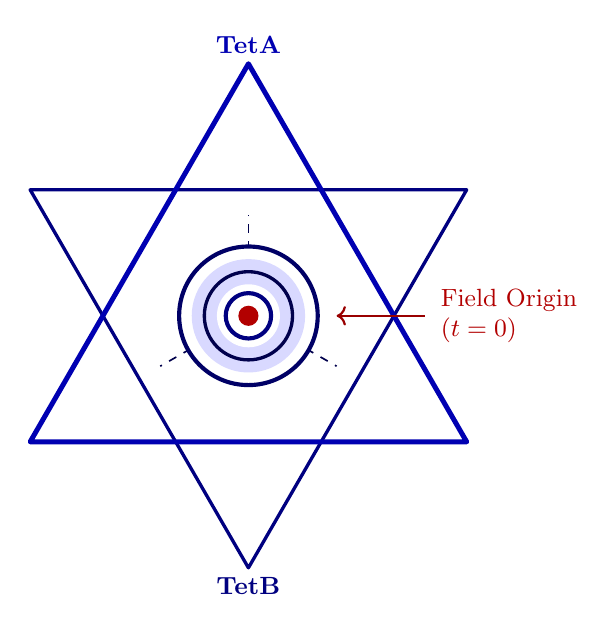
\begin{tikzpicture}[scale=1.6, line join=round]

% Symmetric front-facing stellated octahedron (hexagram view)
% Using regular hexagram geometry for perfect symmetry

% Calculate coordinates for perfect hexagram
% TetA (pointing up) - blue triangle
\coordinate (A0) at (0, 2.0);              % Top apex
\coordinate (A1) at (-1.732, -1.0);        % Bottom-left vertex
\coordinate (A2) at (1.732, -1.0);         % Bottom-right vertex

% TetB (pointing down) - darker blue triangle  
\coordinate (B0) at (0, -2.0);             % Bottom apex
\coordinate (B1) at (-1.732, 1.0);         % Top-left vertex
\coordinate (B2) at (1.732, 1.0);          % Top-right vertex

% Field Origin at center
\coordinate (O) at (0, 0);

% Draw TetB first (pointing down) - slightly thinner lines for depth
\draw[blue!50!black, line width=1.2pt] (B0) -- (B1) -- (B2) -- cycle;

% Draw TetA (pointing up) - thicker lines (front)
\draw[blue!70!black, line width=1.8pt] (A0) -- (A1) -- (A2) -- cycle;

% Add subtle 3D depth lines from center outward (representing edges going into page)
\draw[blue!30!black, line width=0.6pt, dashed] (O) -- (0, 0.8);
\draw[blue!30!black, line width=0.6pt, dashed] (O) -- (-0.7, -0.4);
\draw[blue!30!black, line width=0.6pt, dashed] (O) -- (0.7, -0.4);

% Field Origin - concentric circles like reference image
\fill[white] (O) circle (0.55);
\draw[blue!40!black, line width=1.5pt] (O) circle (0.55);
\fill[blue!15!white] (O) circle (0.45);
\draw[blue!30!black, line width=1.2pt] (O) circle (0.35);
\fill[white] (O) circle (0.25);
\draw[blue!50!black, line width=1.5pt] (O) circle (0.18);
\fill[red!70!black] (O) circle (0.08);

% Label for Field Origin (directly to the right of center)
\draw[->, thick, red!60!black] (1.4, 0) -- (0.7, 0);
\node[font=\small, right, align=left, red!70!black] at (1.45, 0) {Field Origin\\($t = 0$)};

% Label for top apex (TetA)
\node[blue!70!black, font=\small\bfseries, above] at (A0) {TetA};

% Label for bottom apex (TetB)
\node[blue!50!black, font=\small\bfseries, below] at (B0) {TetB};

\end{tikzpicture}
\caption{The stellated octahedron: two tetrahedra with opposite orientations sharing a common center. TetA (thick lines) points upward; TetB (thinner lines) points downward. The structure has 8 vertices (4 from each tetrahedron) and 8 faces (4 per tetrahedron). At the geometric center lies the Field Origin, where the two spacetime sectors couple. This is the $(3+1)^2$ topology from which the fundamental equations derive.}
\label{fig:stellated}
\end{figure}

\subsection{The Field Origin}
\label{subsec:origin}

Bimetric gravity requires that two dynamical metrics interact. But how do they interact? The Hassan-Rosen formulation~\cite{hassan2012} and the vielbein extension by Deffayet, Mourad, and Zahariade~\cite{deffayet2013} establish that the two spin-2 fields must couple at a shared spacetime point, what the literature calls an \emph{interaction vertex}. Without such a vertex, the two metrics would be causally disconnected: two separate gravitational fields with no physical relationship.

The stellated octahedron provides exactly this interaction vertex. At the geometric center, equidistant from all eight vertices, the two tetrahedra share a single point. This is where the two spacetime sectors meet, where information from one tetrahedron can couple to the other. We call this point the \textbf{Field Origin}.

Why does time vanish at this point? Consider the light-travel time from the coupling center to any point at distance $r$. In the local tetrad frame, where spacetime is Minkowski, the propagation time along a radial null geodesic is:
\begin{equation}
\tau_{\text{prop}} = \frac{r}{c}
\end{equation}

At the center itself, $r = 0$:
\begin{equation}
\tau_{\text{prop}} = \frac{0}{c} = 0
\end{equation}

The propagation time vanishes at the Field Origin. But this equation says more than ``time is zero here.'' Read in the other direction, $\tau_{\text{prop}} = r/c$ means time \emph{increases} with distance from the origin. Time radiates outward. The Field Origin is not merely a point where time happens to vanish; it is the source from which all time structure emerges. The analogy is the eye of a hurricane: perfectly still, yet generating the entire storm. The Field Origin has $\tau_{\text{prop}} = 0$ while being the point from which temporal separation radiates into both tetrahedral sectors.

This property is what makes the interaction vertex physically meaningful. The two tetrahedra represent two separate spacetime sectors with opposite orientations. For ghost-free coupling, they must meet at a point where their interaction can be instantaneous, unmediated by propagation delay. The Field Origin, where $\tau_{\text{prop}} = 0$, satisfies this requirement. It is the unique point where the two sectors can exchange information without temporal separation.

The vanishing of temporal separation also bears on quantum entanglement. Entangled particles share a single Field Origin where $\tau_{\text{prop}} = 0$. The correlation between measurements does not travel between the particles; it exists at the shared origin where temporal separation is absent. This is consistent with the observed violation of Bell inequalities without superluminal signaling: no signal is needed because the correlated state resides at a point where time does not elapse.

\subsubsection*{Why everything spins}

One of the deepest questions in physics: why does everything rotate? Stars spin. Galaxies spin. Electrons spin. Angular momentum pervades the universe at every scale. Is this a coincidence, or does it follow from something fundamental?

Einstein-Cartan theory, developed in 1922, provides a hint~\cite{hehl1976}. Cartan showed that spacetime geometry and intrinsic spin are intimately connected: the spin of matter couples directly to spacetime torsion. In this framework, spin is not merely a property that particles happen to have; it is a geometric feature of spacetime itself. Where there is torsion, there is spin. Where there is spin, there is torsion.

The dual tetrahedral structure makes this connection concrete. When two tetrahedra with opposite orientations couple at a shared point, they create a natural rotational flow. One tetrahedron spirals angular momentum inward; the other spirals it outward. The coupling point mediates this exchange. The structure does not merely permit rotation; it \emph{requires} it.

\subsubsection*{The vortex topology}

The Field Origin has a distinctive topology: it is a vortex core. Consider the analogy of water flowing in a river whirlpool (Figure~\ref{fig:vortex}, left panel). At the surface, water spirals inward. As it approaches the center, it accelerates, passes through the central axis, and disperses below. The vortex core is not where motion stops; it is where rotation vanishes but through-flow continues.

The dual tetrahedral structure exhibits the same pattern (Figure~\ref{fig:vortex}, right panel). Angular momentum spirals inward through one tetrahedron (TetA), passes through the Field Origin, and spirals outward through the other (TetB). At the Field Origin itself, the rotational component vanishes (because $t = 0$ there), but the flow of angular momentum continues through. This is the geometric origin of spin: angular momentum flowing through the topological eye of the vortex.

\begin{figure}[H]
\centering
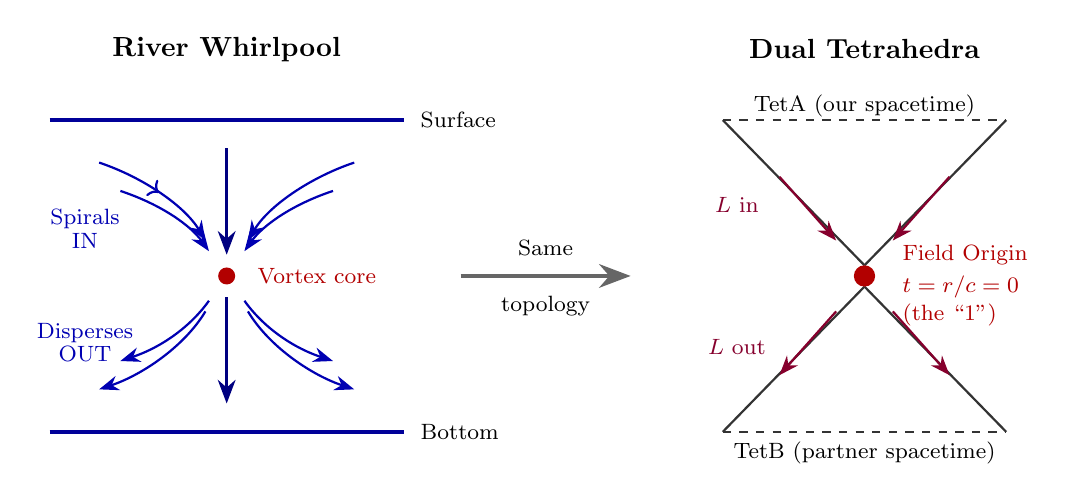
\begin{tikzpicture}[scale=0.9]
% ============================================================
% LEFT PANEL: River Whirlpool
% ============================================================
\begin{scope}[xshift=-4.5cm]
    % Title
    \node[font=\bfseries] at (0,3.2) {River Whirlpool};
    
    % Surface line
    \draw[very thick, blue!60!black] (-2.5,2.2) -- (2.5,2.2);
    \node[font=\footnotesize, right] at (2.6,2.2) {Surface};
    
    % Bottom line
    \draw[very thick, blue!60!black] (-2.5,-2.2) -- (2.5,-2.2);
    \node[font=\footnotesize, right] at (2.6,-2.2) {Bottom};
    
    % Vortex core (central point)
    \fill[red!70!black] (0,0) circle (0.12);
    \node[font=\footnotesize, right, red!70!black] at (0.3,0) {Vortex core};
    
    % Central downward flow (vertical arrow through center)
    \draw[-{Stealth[length=3mm]}, line width=1.2pt, blue!50!black] (0,1.8) -- (0,0.3);
    \draw[-{Stealth[length=3mm]}, line width=1.2pt, blue!50!black] (0,-0.3) -- (0,-1.8);
    
    % Spiral arrows - upper (inward rotation + down)
    % Left side - clockwise approaching
    \draw[-{Stealth[length=2.5mm]}, thick, blue!70!black, 
          decoration={markings, mark=at position 0.5 with {\arrow{>}}}, postaction={decorate}] 
          (-1.8,1.6) .. controls (-1.2,1.4) and (-0.6,1.0) .. (-0.3,0.5);
    \draw[-{Stealth[length=2.5mm]}, thick, blue!70!black] 
          (-1.5,1.2) .. controls (-0.9,1.0) and (-0.5,0.7) .. (-0.25,0.35);
    
    % Right side - clockwise approaching  
    \draw[-{Stealth[length=2.5mm]}, thick, blue!70!black] 
          (1.8,1.6) .. controls (1.2,1.4) and (0.6,1.0) .. (0.3,0.5);
    \draw[-{Stealth[length=2.5mm]}, thick, blue!70!black] 
          (1.5,1.2) .. controls (0.9,1.0) and (0.5,0.7) .. (0.25,0.35);
    
    % Spiral arrows - lower (outward + dispersing)
    % Left side - counterclockwise departing
    \draw[-{Stealth[length=2.5mm]}, thick, blue!70!black] 
          (-0.3,-0.5) .. controls (-0.6,-1.0) and (-1.2,-1.4) .. (-1.8,-1.6);
    \draw[-{Stealth[length=2.5mm]}, thick, blue!70!black] 
          (-0.25,-0.35) .. controls (-0.5,-0.7) and (-0.9,-1.0) .. (-1.5,-1.2);
    
    % Right side - counterclockwise departing
    \draw[-{Stealth[length=2.5mm]}, thick, blue!70!black] 
          (0.3,-0.5) .. controls (0.6,-1.0) and (1.2,-1.4) .. (1.8,-1.6);
    \draw[-{Stealth[length=2.5mm]}, thick, blue!70!black] 
          (0.25,-0.35) .. controls (0.5,-0.7) and (0.9,-1.0) .. (1.5,-1.2);
    
    % Labels
    \node[font=\footnotesize, blue!70!black] at (-2.0,0.8) {Spirals};
    \node[font=\footnotesize, blue!70!black] at (-2.0,0.5) {IN};
    \node[font=\footnotesize, blue!70!black] at (-2.0,-0.8) {Disperses};
    \node[font=\footnotesize, blue!70!black] at (-2.0,-1.1) {OUT};
\end{scope}

% ============================================================
% CENTER: Arrow showing equivalence
% ============================================================
\draw[-{Stealth[length=4mm]}, line width=1.5pt, black!60] (-1.2,0) -- (1.2,0);
\node[font=\footnotesize, above] at (0,0.15) {Same};
\node[font=\footnotesize, below] at (0,-0.15) {topology};

% ============================================================
% RIGHT PANEL: Dual Tetrahedra
% ============================================================
\begin{scope}[xshift=4.5cm]
    % Title
    \node[font=\bfseries] at (0,3.2) {Dual Tetrahedra};
    
    % Upper tetrahedron (TetA) - pointing down
    \draw[thick, black!80] (-2,2.2) -- (0,0.15);
    \draw[thick, black!80] (2,2.2) -- (0,0.15);
    \draw[thick, black!80, dashed] (-2,2.2) -- (2,2.2);
    \node[font=\footnotesize] at (0,2.4) {TetA (our spacetime)};
    
    % Lower tetrahedron (TetB) - pointing up
    \draw[thick, black!80] (-2,-2.2) -- (0,-0.15);
    \draw[thick, black!80] (2,-2.2) -- (0,-0.15);
    \draw[thick, black!80, dashed] (-2,-2.2) -- (2,-2.2);
    \node[font=\footnotesize] at (0,-2.5) {TetB (partner spacetime)};
    
    % Field Origin (central point)
    \fill[red!70!black] (0,0) circle (0.15);
    
    % Field Origin label with box
    \node[font=\footnotesize, right, red!70!black, align=left] at (0.4,0.3) {Field Origin};
    \node[font=\footnotesize, right, red!70!black, align=left] at (0.4,-0.15) {$t = r/c = 0$};
    \node[font=\footnotesize, right, red!70!black, align=left] at (0.4,-0.55) {(the ``1'')};
    
    % Angular momentum flow arrows
    \draw[-{Stealth[length=2.5mm]}, thick, purple!70!black] (-1.2,1.4) -- (-0.4,0.5);
    \draw[-{Stealth[length=2.5mm]}, thick, purple!70!black] (1.2,1.4) -- (0.4,0.5);
    \draw[-{Stealth[length=2.5mm]}, thick, purple!70!black] (-0.4,-0.5) -- (-1.2,-1.4);
    \draw[-{Stealth[length=2.5mm]}, thick, purple!70!black] (0.4,-0.5) -- (1.2,-1.4);
    
    % Labels for flow
    \node[font=\footnotesize, purple!70!black] at (-1.8,1.0) {$L$ in};
    \node[font=\footnotesize, purple!70!black] at (-1.8,-1.0) {$L$ out};
\end{scope}

\end{tikzpicture}
\caption{The Field Origin as a vortex core. \textbf{Left:} A river whirlpool viewed from the side. Water spirals inward at the surface, passes through the central axis, and disperses below. At the vortex core, rotation vanishes but through-flow continues. \textbf{Right:} The dual tetrahedral structure. Angular momentum spirals inward through TetA, passes through the Field Origin where $t = 0$, and spirals outward through TetB. At both vortex cores, rotation $\to 0$ but flow continues through. At the Field Origin, proper time $\tau \to 0$, yet angular momentum flows through, yielding the observed spin $\hbar/2$.}
\label{fig:vortex}
\end{figure}

\subsubsection*{Why spin equals $\hbar/2$}

The vortex structure explains not just that electrons spin, but why they spin with exactly the value $\hbar/2$. The companion paper~\cite{paper6} derived this from the geometry:
\begin{equation}
S = \frac{N_{\text{TIME}}}{N_{\text{total}}} \times L_{\text{total}} = \frac{2}{8} \times 2\hbar = \frac{\hbar}{2}
\label{eq:spin}
\end{equation}

The derivation has two inputs: one from quantum mechanics and one from topology. The quantum-mechanical input is that closed loops carry quantized angular momentum in units of $\hbar$. This is standard physics, not derived here. A complete circuit through all four faces of a tetrahedron constitutes a closed loop, carrying angular momentum $\hbar$; the stellated octahedron (two tetrahedra) therefore carries total angular momentum $2\hbar$.

What the topology uniquely determines is the \emph{fraction}. Not all angular momentum passes through the Field Origin. Only 2 of the 8 faces are TIME faces, those pointing toward the vortex core (Section~\ref{subsec:faces} will develop this in detail). The remaining 6 SPATIAL faces point outward and carry orbital angular momentum. The observable intrinsic spin is the fraction that flows through the topological eye: $(2/8) \times 2\hbar = \hbar/2$.

The face ratio $2/8 = 1/4$ is a geometric fact about the stellated octahedron; it is not adjustable and does not appear in any other theoretical framework. The vortex eye is an aperture: it admits angular momentum only through the 2 faces that point toward it, filtering out the 6 that point away. Spin $\hbar/2$ is the throughput of this aperture, the portion of total angular momentum that passes through the topological eye. Given quantized angular momentum (standard QM), the topology determines which fraction constitutes intrinsic spin.

\subsection{The Face Structure}
\label{subsec:faces}

Each tetrahedron has 4 faces. In the stellated octahedron, these 8 faces divide into two types based on their orientation relative to the Field Origin:

\begin{itemize}
\item \textbf{TIME faces} (2 total): The face opposite each apex points inward, toward the Field Origin. These faces connect to the coupling point where $t = 0$. They are called TIME faces because they point toward the temporal origin.
\item \textbf{SPATIAL faces} (6 total): The three faces sharing each apex point outward, toward external space. These faces radiate away from the origin into the spatial dimensions.
\end{itemize}

The ratio 2:6, or equivalently 2/8 of the total faces pointing inward, is fixed by the geometry. This ratio has physical consequences. Angular momentum, like all physical quantities in this framework, must pass through the Field Origin to be measured. Only the component of angular momentum aligned with the TIME faces, the faces pointing toward the coupling point, can be observed. The 2/8 ratio therefore determines what fraction of total angular momentum is measurable, and this will yield electron spin.

\subsection{The Coupling Hierarchy}
\label{subsec:hierarchy}

The structure (3+1) denotes three spatial dimensions plus one time dimension: ordinary spacetime. With two coupled tetrahedra, we have (3+1)$^2$: two spacetimes interacting.

But coupling between the two tetrahedra does not happen all at once. It has levels, each contributing to the total interaction strength. Consider what must connect for gravity to operate:

\begin{enumerate}
\item \textbf{The Field Origin itself (contributes ``1'').} Coupling begins at the origin, where the two tetrahedra meet. This is the foundation: without the origin, there is no coupling at all.
\item \textbf{One complete spacetime (contributes ``4'').} From the origin, the field extends through one tetrahedron's (3+1) structure: 3 spatial dimensions plus 1 time dimension. This is how one side of the coupling propagates.
\item \textbf{The full bimetric interaction (contributes ``16'').} Both tetrahedra interact fully. Each has (3+1) dimensions, so the complete interaction space is $(3+1) \times (3+1) = 16$-dimensional.
\end{enumerate}

The total coupling hierarchy is:
\begin{equation}
1 + (3+1) + (3+1)^2 = 1 + 4 + 16 = 21
\label{eq:hierarchy}
\end{equation}

This number, 21, will appear as the exponent in the gravitational constant. Read as a narrative, the hierarchy tells a story: begin at the source of time (the ``1''), from which spacetime radiates outward ((3+1)), and through which the two spacetime sectors couple to each other $((3+1)^2)$. Gravity must traverse this entire chain. Without the origin, there is no source. Without the source, there is no spacetime. Without two spacetimes, there is no coupling. The exponent 21 counts every channel in this chain.

\subsubsection*{Clarification: the ``1'' versus the ``$+1$''}

The hierarchy contains a ``1'' and the spacetime structure contains a ``$+1$.'' These are related but distinct.

The ``$+1$'' in $(3+1)$ represents time as a \emph{dimension}. It exists everywhere in spacetime; every point in the universe has a time coordinate. This is what distinguishes spacetime from ordinary three-dimensional space.

The standalone ``1'' in the hierarchy represents time's \emph{origin}, the specific point where the time coordinate equals zero. The distinction is analogous to ``the $x$-axis'' (a dimension extending everywhere) versus ``$x = 0$'' (a specific point on that axis).

\begin{table}[H]
\centering
\begin{tabular*}{0.95\textwidth}{@{\extracolsep{\fill}} lll @{}}
\toprule
\textbf{Symbol} & \textbf{What it represents} & \textbf{Where it applies} \\
\midrule
The ``$+1$'' in $(3+1)$ & Time as a dimension & Throughout spacetime \\
The ``1'' in the hierarchy & Time's origin & At $r = 0$, where $t = r/c = 0$ \\
\bottomrule
\end{tabular*}
\caption{The distinction between time as dimension and time's origin.}
\label{tab:one-vs-plusone}
\end{table}

The companion paper~\cite{paper6} identified the ``1'' with time. This identification was correct; the present clarification specifies: the ``1'' is where time equals zero.

\subsubsection*{Why the hierarchy explains $E = mc^2$}

The coupling hierarchy not only counts channels; it explains why Einstein's equation takes the form $E = mc^2$.

Consider where mass exists in this structure. Mass is energy that does not propagate: a photon (massless) travels at $c$, while a massive particle at rest remains localized. In the tetrahedral framework, mass is energy bound at the Field Origin, the ``1'' where the two tetrahedra couple and where $\tau_{\text{prop}} = 0$. The binding mechanism is topological: energy at the coupling point is shared between the two tetrahedra simultaneously, with each sector's boundary conditions preventing the energy from propagating outward through either one alone. A particle with mass is a stable configuration of energy localized at this coupling point.

Now consider what happens during mass-energy conversion. Energy stored at the Field Origin must propagate outward. But outward through what? Through both tetrahedra. The structure is $(3+1)^2$, not $(3+1)$. Two spacetimes, not one.

Each tetrahedron propagates disturbances at the closure speed, the speed at which field consistency is maintained. Lorentz invariance requires this speed to equal $c$: any finite propagation speed for a fundamental field must be the invariant speed, since a frame-dependent closure speed would violate the equivalence principle. The $c$ speed limit is therefore not a traffic law imposed on objects moving through space; it is the processing speed of the spacetime structure itself. Exceeding $c$ would mean outrunning the very field that defines one's existence. When energy leaves the Field Origin, it engages both:
\begin{equation}
E = m \times c_{\text{TetA}} \times c_{\text{TetB}} = m \times c \times c = mc^2
\end{equation}

The ``squared'' in $c^2$ has the same origin as the ``squared'' in $(3+1)^2$: both reflect the bimetric structure. This provides a geometric interpretation of why mass-energy conversion involves $c^2$ rather than some other power. The standard derivation from Lorentz invariance establishes that $c^2$ is required; the $(3+1)^2$ topology suggests \emph{why} spacetime has the structure that produces this requirement.

The hierarchy thus answers three questions simultaneously:
\begin{enumerate}
\item \textbf{Where is mass?} At the ``1'' (the Field Origin, where $t = 0$)
\item \textbf{Why does conversion involve $c$?} Because each tetrahedron has closure speed $c$
\item \textbf{Why $c^2$?} Because $(3+1)^2$ means two tetrahedra, hence $c \times c$
\end{enumerate}

Einstein's equation is not separate from the coupling hierarchy. It is a direct reading of the $(3+1)^2$ structure: mass at the origin, conversion through two spacetimes, $c^2$ from two closure speeds.

With the foundation established, we can now derive the equations.

% ============================================================================
% SECTION 4: THE (3+1) EQUATIONS
% ============================================================================
\section{The (3+1) Equations}
\label{sec:five}

This section presents the four equations that emerge from the $(3+1)^2$ topology. We begin at the center: $G$ from tetrad topology, which encodes the $(3+1)$ structure in every term. The ``1'' that appears four times is the Field Origin, where $t = 0$. From this center, three fundamental relationships radiate outward: the inverse square law (unifying Newton and Coulomb), mass-energy equivalence (explaining why $c$ appears squared), and the force hierarchy (resolving the $10^{-43}$ ratio).

\subsection{$G$ from Tetrad Topology}
\label{subsec:master-eq}

The equation for $G$ encodes the $(3+1)$ structure in every term. The companion paper~\cite{paper6} derived the gravitational constant; here we make the underlying geometry visible. The equation contains a deep insight: the ``1'' that appears four times is the Field Origin, where $t = 0$.

\subsubsection*{Where time vanishes and originates}

Section~\ref{subsec:origin} established that $\tau_{\text{prop}} = r/c = 0$ at the Field Origin, and that the origin is not merely where time vanishes but the source from which time radiates outward. The zero \emph{is} the source.

\subsubsection*{The equation for $G$}

The gravitational constant, derived in the companion paper~\cite{paper6}, can be written with the $(3+1)$ structure visible in every component:

\vspace{1.5em}
\noindent
\colorbox{resultgreen}{\parbox{\dimexpr\textwidth-2\fboxsep\relax}{%
\vspace{0.8em}
\centering
\textbf{\large Result 1: $G$ from Tetrad Topology}

\vspace{0.5em}
\boldmath
\begin{equation}
G = \frac{(3+\mathbf{1})^2 + \mathbf{1}}{3(3+\mathbf{1}) + \mathbf{1}} \times \alpha^{\mathbf{1}+(3+1)+(3+1)^2} \times \frac{\hbar c}{m_e^2}
\label{eq:master}
\end{equation}
\unboldmath

\vspace{0.3em}
Predicted: $\bm{6.666 \times 10^{-11}}$~m$^3$/(kg$\cdot$s$^2$) \quad Measured: $6.674 \times 10^{-11}$~m$^3$/(kg$\cdot$s$^2$)

\textbf{Agreement: 0.12\%}
\vspace{0.5em}
}}
\vspace{1cm}

The 0.12\% deviation merits comment. The gravitational constant is the least precisely measured fundamental constant, with inter-experiment scatter of $\sim$0.05\% and CODATA relative uncertainty of 22~ppm. The predicted deviation exceeds both, suggesting either (a)~a higher-order correction the topology does not yet capture, analogous to QED corrections to the electron $g-2$, or (b)~systematic effects in measurements that future experiments may resolve. This is a falsifiable prediction: if precision measurements converge on a value outside the $\sim$0.1\% window, the topological formula would require revision.

\textbf{Sensitivity of the exponent.} The exponent $1 + (3+1) + (3+1)^2 = 21$ is not one of many workable values. Each unit change multiplies the prediction by $1/\alpha \approx 137$:

\begin{center}
\begin{tabular}{ccc}
\toprule
\textbf{Exponent} & \textbf{Predicted $G$} & \textbf{Deviation from measurement} \\
\midrule
20 & $9.1 \times 10^{-9}$ & $\times 137$ too large \\
\textbf{21} & $\bm{6.67 \times 10^{-11}}$ & \textbf{0.12\%} \\
22 & $4.9 \times 10^{-13}$ & $\times 137$ too small \\
\bottomrule
\end{tabular}
\end{center}

Adjacent integers miss by over two orders of magnitude. The agreement at 21 is not insensitive to the exponent; it is sharply selective. The value $21 = 1 + 4 + 16$ is the only integer in the vicinity that produces a physically reasonable gravitational constant.

The expanded form reveals the underlying geometry; every factor traces to the $(3+1)$ structure of spacetime. In fact, the entire equation is determined by a single integer, the spatial dimension $d$:
\begin{equation}
G = \frac{(d+1)^2 + 1}{3(d+1) + 1} \times \alpha^{1 + (d+1) + (d+1)^2} \times \frac{\hbar c}{m_e^2}
\label{eq:G-general-d}
\end{equation}
Setting $d = 3$ produces the prefactor 17/13, the exponent 21, and the observed gravitational constant. No other value of $d$ yields a universe with both stable orbits and stable atoms (Section~\ref{subsec:inverse-square}).

\subsubsection*{The four ``1''s}

The equation for $G$ contains four distinct appearances of ``1,'' each representing the Field Origin from a different perspective:

\begin{table}[H]
\centering
\begin{tabular*}{\textwidth}{@{\extracolsep{\fill}} llll @{}}
\toprule
\textbf{Location} & \textbf{Expression} & \textbf{Value} & \textbf{Physical meaning} \\
\midrule
Exponent start & $\mathbf{1} + 4 + 16$ & 21 & The Field Origin ($t = 0$), source of hierarchy \\
Spacetime structure & $3 + \mathbf{1}$ & 4 & 3 space + 1 time radiating from origin \\
Numerator & $16 + \mathbf{1}$ & 17 & Bimetric channels + origin as coupling interface \\
Denominator & $12 + \mathbf{1}$ & 13 & Spatial couplings + origin as structural base \\
\bottomrule
\end{tabular*}
\caption{The four appearances of ``1'' in the equation for $G$.}
\label{tab:ones}
\end{table}

Every ``1'' is the same geometric object viewed from a different angle: the Field Origin where $t = 0$, where the two tetrahedra couple, where gravity's hierarchy begins.

\subsubsection*{The hierarchy as narrative}

The exponent $1 + (3+1) + (3+1)^2 = 21$ is not merely arithmetic. It tells a story:

\begin{enumerate}
\item \textbf{The origin (1):} Start at the Field Origin, where $t = 0$. This is the source.
\item \textbf{One spacetime (3+1):} From the origin, spacetime radiates outward. Three spatial dimensions plus one time dimension.
\item \textbf{Bimetric coupling (3+1)$^2$:} Both tetrahedra interact. The full $(3+1) \times (3+1) = 16$-dimensional coupling engages.
\end{enumerate}

Gravity couples through all 21 levels. Electromagnetism couples only at level 1. The force hierarchy (Section~\ref{subsec:hierarchy-eq}) follows directly from this narrative.

\subsubsection*{How the equation encodes all four results}

The equation for $G$ is one geometric structure with four readable consequences:

\textbf{Dimensionality $\rightarrow$ inverse square law.} The $(3+1)$ in the prefactor reflects four faces per tetrahedron, the minimal simplex in $d = 3$ dimensions. The same three-dimensionality produces $1/r^2$ through field spreading (Section~\ref{subsec:inverse-square}).

\textbf{Bimetric structure $\rightarrow$ $c^2$.} The scale $\hbar c/m_e^2$ contains $c$ in the numerator. The bimetric structure, requiring two tetrahedra with closure speed $c$ each, explains why mass-energy conversion involves $c \times c = c^2$ (Section~\ref{subsec:emc2}).

\textbf{Coupling levels $\rightarrow$ force hierarchy.} The exponent 21 encodes the full hierarchy. Gravity traverses all levels; electromagnetism uses 1. The ratio $\alpha^{20} \approx 10^{-43}$ follows (Section~\ref{subsec:hierarchy-eq}).

\textbf{Complete equation $\rightarrow$ $G$.} Combining the $(3+1)$ prefactor, coupling ($\alpha^{21}$), and scale ($\hbar c/m_e^2$) yields $G$ to 0.12\% accuracy.

\subsubsection*{The origin unifies everything}

The Field Origin is not incidental. It is the reason gravity exists:
\begin{itemize}
\item Without the origin: no $t = 0$ point, no source for time
\item Without the coupling point: no bimetric interaction
\item Without the ``1'' in the exponent: no hierarchy
\end{itemize}

The $(3+1)^2$ structure is self-consistent. The number $(3+1)$ appears in the dimensions, in the faces, in the prefactor, and in the exponent. The ``1'' appears as time, as origin, as coupling interface, and as structural foundation. This result does not merely calculate $G$; it encodes the geometry of spacetime itself.

The three sections that follow unpack the consequences that radiate from this center.

\subsection{The Inverse Square Law}
\label{subsec:inverse-square}

Newton's gravitational force and Coulomb's electrostatic force share an identical spatial form: both decrease as $1/r^2$. This coincidence has persisted for centuries without geometric explanation. Why do two apparently different forces follow the same distance dependence?

The $(3+1)^2$ topology provides the answer through dimensional geometry. The tetrahedron is the minimal solid in three dimensions: it has $d + 1 = 4$ vertices and faces for $d = 3$ spatial dimensions. This relationship between the simplex and dimensionality is fixed by geometry.

Why does space have three dimensions? The answer is physical stability. In $d = 2$ dimensions, the gravitational force law $F \propto 1/r$ cannot produce stable closed orbits (Bertrand's theorem~\cite{goldstein2002} permits closed orbits only for $1/r^2$ and $r^2$ potentials). In $d \geq 4$ dimensions, the force law $F \propto 1/r^{d-1}$ is too steep: the hydrogen atom has no bound states because the centrifugal barrier cannot prevent collapse. Only $d = 3$ permits both stable orbits and stable matter. Given $d = 3$, the simplex is the tetrahedron with 4 faces. Given the tetrahedron, the $(3+1)^2$ topology follows from the stability requirements of Section~\ref{subsec:two-tet}.

In three-dimensional space, any field emanating from a point source spreads over a spherical surface. The area of that surface at distance $r$ is $4\pi r^2$. If field strength is conserved (flux through any enclosing surface is constant), then intensity at distance $r$ must decrease as the area increases: intensity $\propto 1/r^2$.

The inverse square law is not a separate physical principle. It is the geometry of three-dimensional space. The same $d = 3$ that requires the tetrahedron also produces $1/r^2$.

\vspace{1.5em}
\noindent
\colorbox{resultgreen}{\parbox{\dimexpr\textwidth-2\fboxsep\relax}{%
\vspace{0.8em}
\centering
\textbf{\large Result 2: The Inverse Square Law}

\vspace{0.5em}
\boldmath
\begin{equation}
F \propto \frac{1}{r^2} \quad \text{(for both gravity and electromagnetism)}
\end{equation}
\unboldmath

\vspace{0.3em}
Field spreading in three-dimensional space produces $1/r^2$ universally. The tetrahedron's four faces reflect the same $d = 3$.
\vspace{0.5em}
}}
\vspace{1cm}

This result unifies Newton and Coulomb. Both wrote:
\begin{align}
F_{\text{Newton}} &= G\frac{m_1 m_2}{r^2} \\[0.5em]
F_{\text{Coulomb}} &= k\frac{q_1 q_2}{r^2}
\end{align}

The $1/r^2$ dependence is identical. Only the prefactors ($G$ versus $k$) and the sources (mass versus charge) differ. Electromagnetism and gravity are geometric siblings: both obey $1/r^2$ because both propagate through three-dimensional space from the same tetrahedral coupling structure, differing only in coupling depth ($\alpha^1$ versus $\alpha^{21}$). The inverse square law is not two separate empirical discoveries; it is one geometric consequence of three-dimensional space.

The companion paper derived the gravitational constant formula~\cite{paper6}, where the prefactor $[(3+1)^2+1]/[3(3+1)+1]$ counts coupling channels over structural elements in the dual tetrahedral geometry. The $1/r^2$ spatial dependence derived here is complementary: the prefactor determines the \emph{strength}, while three-dimensional spreading determines the \emph{form}. Together they explain Newton's complete equation.

\subsection{Mass-Energy Equivalence}
\label{subsec:emc2}

Section~\ref{subsec:hierarchy} established why $E = mc^2$ takes this form: mass is energy bound at the Field Origin (the ``1''), and conversion engages both tetrahedra, each with closure speed $c$. The ``squared'' in $c^2$ has the same origin as the ``squared'' in $(3+1)^2$. Here we present this as a formal result and trace its connection to $G$ from tetrad topology.

\vspace{1.5em}
\noindent
\colorbox{resultgreen}{\parbox{\dimexpr\textwidth-2\fboxsep\relax}{%
\vspace{0.8em}
\centering
\textbf{\large Result 3: Mass-Energy Equivalence}

\vspace{0.5em}
\boldmath
\begin{equation}
E = m \times c_{\text{TetA}} \times c_{\text{TetB}} = m \times c \times c = mc^2
\end{equation}
\unboldmath

\vspace{0.3em}
The $c^2$ factor is the product of two closure speeds, one from each tetrahedron.
\vspace{0.5em}
}}
\vspace{1cm}

The speed $c$ appears in both Einstein's mass-energy relation and Maxwell's electromagnetic equations. In the $(3+1)^2$ framework, this is not coincidence: both emerge from the closure speed of the tetrahedral structure. Any field propagating through the $(3+1)$ topology must travel at $c$, whether it carries gravitational, electromagnetic, or any other interaction.

This result connects directly to the topological derivation of $G$. The formula contains $c$ in the numerator (via $\hbar c$) and $m_e^2$ in the denominator. Both appearances trace to the same bimetric source:

\begin{itemize}
\item The $c$ in $\hbar c$ reflects one closure speed (field propagation)
\item The $m_e^2$ in the denominator reflects energy bound at the Field Origin, squared because both tetrahedra participate
\end{itemize}

Einstein's $c^2$ and the $\hbar c/m_e^2$ scale in $G$ share the same geometric origin: the two-tetrahedron structure requires two factors wherever mass or energy crosses between the bimetric sectors. The closure speed also explains why $c$ is the universal speed limit: in the $(3+1)$ structure, every object moves through spacetime at the invariant speed $c$, partitioned as $c^2 = v_{\text{space}}^2 + v_{\text{time}}^2$. Moving faster through space leaves less budget for moving through time, which is why clocks slow at high velocities and stop entirely at $v = c$.

\subsection{The Force Hierarchy}
\label{subsec:hierarchy-eq}

Section~\ref{subsec:inverse-square} established that Newton's gravity and Coulomb's electromagnetism share the same spatial form: $F \propto 1/r^2$. Yet gravity is approximately $10^{43}$ times weaker. If the geometry is identical, why do the strengths differ by such an enormous factor?

The answer lies not in spatial form but in coupling depth, the number of structural levels a force must traverse to complete its interaction. Think of coupling depth as floors in a building: a signal that must pass through more floors arrives weaker at the other end. The $(3+1)^2$ topology contains a hierarchy of coupling channels, established in Section~\ref{subsec:hierarchy}: the Field Origin (1 channel), spacetime (4 channels), and full bimetric interaction (16 channels), totaling 21. Different forces engage different numbers of these channels.

The difference between electromagnetism and gravity lies in what they couple. Electromagnetic interactions involve charge, which exists within a single spacetime. A photon couples to a charged particle at one point in one tetrahedron's structure. This physical picture suggests that electromagnetism engages only the origin channel, giving coupling strength proportional to $\alpha^1$. This assignment is motivated by the physical distinction between local (EM) and bimetric (gravitational) coupling; the numerical match to the observed hierarchy provides empirical support.

Gravitational interactions involve mass, and mass is energy bound at the Field Origin, where both tetrahedra meet. Gravity must therefore couple through the complete bimetric structure: the origin (1 channel), one complete spacetime (4 channels), and the full $(3+1) \times (3+1)$ cross-coupling between both tetrahedra (16 channels). The coupling strength is proportional to $\alpha^{21}$.

\vspace{1.5em}
\noindent
\colorbox{resultgreen}{\parbox{\dimexpr\textwidth-2\fboxsep\relax}{%
\vspace{0.8em}
\centering
\textbf{\large Result 4: The Force Hierarchy}

\vspace{0.5em}
\boldmath
\begin{equation}
\frac{\text{Gravity}}{\text{EM}} \sim \frac{\alpha^{21}}{\alpha^1} = \alpha^{20} \approx \left(\frac{1}{137}\right)^{20} \approx 10^{-43}
\end{equation}
\unboldmath

\vspace{0.3em}
Same spatial form ($1/r^2$), different coupling depth (21 vs.\ 1).
\vspace{0.5em}
}}
\vspace{1cm}

The hierarchy dissolves. Gravity is not mysteriously weak. It is naturally attenuated because it must traverse the complete geometric hierarchy: 21 coupling channels versus electromagnetism's single channel. The 20-order difference in coupling exponents produces the 43-order difference in observed strength. No fine-tuning is required; the ratio follows from counting levels in the $(3+1)^2$ topology.

This result completes the connection between Newton and Maxwell. Both forces follow $1/r^2$ because both propagate through three-dimensional space (Section~\ref{subsec:inverse-square}). They differ in strength because electromagnetism couples locally while gravity engages the full bimetric hierarchy. The spatial form is shared; the coupling depth is distinct.

% ============================================================================
% ============================================================================
% SECTION 5: QUANTUM CONSISTENCY
% ============================================================================
\section{Quantum Consistency of the $(3+1)^2$ Topology}
\label{sec:four-more}

Section~\ref{sec:five} derived quantitative predictions from the $(3+1)^2$ topology: $G$ to 0.12\%, the force hierarchy from coupling depth, and the geometric origins of $1/r^2$ and $E = mc^2$. A natural question follows: is the same topology consistent with quantum mechanics?

The $(3+1)^2$ structure operates at the scale of the electron radius, deep within the quantum regime. A geometry that determines $G$ at this scale would be expected to constrain quantum behavior at the same scale. This section examines four aspects of quantum physics through the topological lens. The first, the uncertainty principle, involves a genuinely novel geometric observation (the face ratio). The second, energy quantization, provides a conceptual mechanism. The third and fourth, wave-particle duality and the energy-momentum relation, demonstrate that the topology is consistent with established relativistic quantum mechanics. These vary in rigor; the section is transparent about what is derived, what is interpreted, and what is inherited from standard physics.

\subsection{The Uncertainty Principle}
\label{subsec:uncertainty}

Heisenberg's uncertainty principle states that position and momentum cannot both be known exactly. The more precisely one is measured, the more uncertain the other becomes. This is not a limitation of instruments or experimental technique. It is built into reality.

The mathematical statement is:
\begin{equation}
\Delta x \cdot \Delta p \geq \frac{\hbar}{2}
\end{equation}

The question that persisted for a century: why is the minimum uncertainty exactly $\hbar/2$? Why not $\hbar$, or $2\hbar$, or some other value?

The $(3+1)^2$ framework provides a geometric interpretation. The minimum uncertainty $\hbar/2$ is the same quantity that determines electron spin. In the companion paper~\cite{paper6}, spin was derived from the face ratio of the stellated octahedron: only 2 of the 8 faces point inward toward the Field Origin (the TIME faces); the other 6 point outward. Angular momentum observable through the coupling point is therefore a fraction of the total. As established in Section~\ref{subsec:origin}, each tetrahedron carries angular momentum $\hbar$, giving total $2\hbar$. Only the fraction $(2/8) = 1/4$ can pass through the TIME faces, yielding observable spin $(2/8) \times 2\hbar = \hbar/2$. The same face structure that determines spin-1/2 also determines the minimum observable action. Both are set by the 2/8 aperture of the vortex core: only the TIME-face fraction of angular information passes through the coupling point. The minimum uncertainty $\hbar/2$ and the electron spin $\hbar/2$ share a common geometric origin in the stellated octahedron's face ratio. A rigorous derivation connecting this face ratio to the canonical commutation relation $[\hat{x}, \hat{p}] = i\hbar$ remains an open problem; the geometric argument presented here identifies the structural origin of the $\hbar/2$ scale without yet deriving the full operator algebra.

\vspace{1.5em}
\noindent
\colorbox{resultgreen}{\parbox{\dimexpr\textwidth-2\fboxsep\relax}{%
\vspace{0.8em}
\centering
\textbf{\large Result 5: The Uncertainty Principle}

\vspace{0.5em}
\boldmath
\begin{equation}
\Delta x \cdot \Delta p \geq \frac{\hbar}{2}
\end{equation}
\unboldmath

\vspace{0.3em}
The minimum uncertainty $\hbar/2$ is the spin quantum from the stellated octahedron face ratio.
\vspace{0.5em}
}}
\vspace{1cm}

The physical interpretation follows from the Field Origin. All information passes through the coupling point at the center of the stellated octahedron, where $\tau_{\text{prop}} = 0$. The coupling point has finite angular resolution: only the 2 TIME faces (out of 8 total) mediate the transfer of information between the two tetrahedral sectors. This 2/8 ratio sets the minimum action that any measurement can extract from the structure, namely $\hbar/2$. Position and momentum cannot be resolved below this scale because any observation must pass through the coupling point, and the coupling point transmits only a fraction $1/4$ of the total angular information.

Uncertainty is not ignorance. It is geometry. The universe is not hiding information below the $\hbar/2$ scale; the information genuinely does not exist at that resolution, just as a digital image contains no detail smaller than one pixel. The TIME-face aperture sets the pixel size of reality. The same face structure that produces spin also produces the fundamental limit on what can be simultaneously known.

\subsection{Energy Quantization}
\label{subsec:quantization}

Classical physics assumed energy was continuous: any amount could exist. Experiments revealed otherwise. Heated objects emit light in discrete colors. Atoms absorb only specific frequencies. Energy comes in packets.

Planck's relation captures this:
\begin{equation}
E = hf
\end{equation}

where $h$ is Planck's constant and $f$ is frequency. But this equation was introduced empirically. Planck called it ``an act of desperation''~\cite{planck1931}. The question remained: why is energy quantized?

The $(3+1)^2$ framework provides a conceptual answer through resonance. The Field Origin acts as a topological boundary condition. Consider a guitar string: fixed endpoints permit only standing waves with specific wavelengths. Similarly, the Field Origin's structure selects which field configurations can stably exist. Configurations that do not ``fit'' the boundary cannot persist as stable resonances. This does not derive the value of $h$ from topology, but it explains \emph{why} quantization occurs: discrete modes are the only stable solutions.

Just as a guitar string's length determines which harmonics can sound, the Field Origin's topology determines which frequencies are allowed. The discrete frequencies that satisfy this boundary condition correspond to quantized energies through $E = hf$. Intermediate configurations, those that violate the boundary condition, cannot exist as stable modes. The Field Origin is the universal boundary that selects allowed resonances.

\vspace{1.5em}
\noindent
\colorbox{resultgreen}{\parbox{\dimexpr\textwidth-2\fboxsep\relax}{%
\vspace{0.8em}
\centering
\textbf{\large Result 6: Energy Quantization}

\vspace{0.5em}
\boldmath
\begin{equation}
E = hf
\end{equation}
\unboldmath

\vspace{0.3em}
The Field Origin selects discrete resonance modes. Energy is quantized because only standing waves that fit the origin can exist.
\vspace{0.5em}
}}
\vspace{1cm}

Planck's constant $h = 6.626 \times 10^{-34}$~J$\cdot$s is small because the Field Origin is at the smallest scale. It represents the ``grain size'' of resonance, the minimum action required for one complete cycle at the coupling point. A wave oscillating $f$ times per second completes $f$ cycles in one second. Each cycle requires action $h$ to execute. The energy of such a wave is therefore $E = hf$: action per cycle times cycles per second.

Quantization is not strange. It is what resonance does. Guitar strings have harmonic series. Organ pipes produce specific notes. Atoms have discrete energy levels. The Field Origin is the universal boundary that selects allowed modes.

\subsection{Wave-Particle Duality}
\label{subsec:debroglie}

Light sometimes behaves as a wave (interference, diffraction) and sometimes as a particle (photoelectric effect, Compton scattering). Matter exhibits the same duality: electrons diffract through crystals like waves, yet they register as discrete hits on detectors. De Broglie proposed that every particle has an associated wavelength:
\begin{equation}
\lambda = \frac{h}{p}
\end{equation}

where $p$ is momentum. This relation bridged quantum and classical physics. But it appeared as a postulate, unexplained.

The $(3+1)^2$ framework shows that wave-particle duality is a consequence, not an assumption. From the preceding results, energy is quantized: $E = hf$. For light, we also know that photons are massless and travel at speed $c$. A photon's energy is entirely kinetic, carried by its momentum: $E = pc$. (This is the massless limit of the general energy-momentum relation derived in Section~\ref{subsec:energy-momentum}.)

Combining quantization with the photon relation:
\begin{align}
E &= hf = pc \\
h \cdot \frac{c}{\lambda} &= pc \\
\lambda &= \frac{h}{p}
\end{align}

De Broglie's insight was that this relation applies not just to photons but to all particles. Once the Field Origin selects discrete energy modes and the bimetric structure sets the energy-momentum relation, wave-particle duality emerges automatically. Every particle with momentum $p$ has an associated wavelength $\lambda = h/p$.

\vspace{1em}
\noindent
\fbox{\parbox{\dimexpr\textwidth-2\fboxsep\relax}{%
\vspace{0.5em}
\centering
\textbf{Consistency Check: Wave-Particle Duality}

\vspace{0.3em}
\begin{equation}
\lambda = \frac{h}{p}
\end{equation}

\vspace{0.1em}
De Broglie's relation follows algebraically from quantization ($E = hf$) combined with the relativistic energy-momentum relation. The topology contributes indirectly through the boundary conditions that produce quantization; the algebraic step is standard physics.
\vspace{0.5em}
}}
\vspace{1cm}

The physical picture: a ``particle'' is a resonance at a Field Origin. A ``wave'' is how that resonance propagates through $(3+1)$ space. They are not contradictory. They are two aspects of the same phenomenon. Detection (particle behavior) occurs at the Field Origin. Propagation (wave behavior) occurs through the surrounding spacetime. The duality reflects the structure: localized origin, extended field.

\subsection{The Energy-Momentum Relation}
\label{subsec:energy-momentum}

Section~\ref{subsec:emc2} derived $E = mc^2$ from the bimetric structure: two tetrahedra, each with closure speed $c$, producing $c^2$. But $E = mc^2$ applies only to objects at rest. Moving objects have both rest mass energy and kinetic energy. What is the complete relationship?

Einstein's energy-momentum relation answers:
\begin{equation}
E^2 = (pc)^2 + (m_0 c^2)^2
\end{equation}

This equation has the structure of the Pythagorean theorem in energy-momentum space. Rest mass energy $m_0 c^2$ and momentum contribution $pc$ combine as orthogonal components. Total energy $E$ is the hypotenuse.

Why does energy-momentum follow Pythagorean geometry? The $(3+1)^2$ framework provides the answer: the invariant interval.

\vspace{1em}
\noindent
\fbox{\parbox{\dimexpr\textwidth-2\fboxsep\relax}{%
\vspace{0.5em}
\centering
\textbf{Consistency Check: The Energy-Momentum Relation}

\vspace{0.3em}
\begin{equation}
E^2 = (pc)^2 + (m_0 c^2)^2
\end{equation}

\vspace{0.1em}
The energy-momentum relation follows from the invariance of the $(3+1)$ spacetime interval. The topology provides the $(3+1)$ structure; the Pythagorean form follows from Lorentz invariance, which is standard special relativity.
\vspace{0.5em}
}}
\vspace{1cm}

The derivation follows from the spacetime interval. In the $(3+1)$ structure, the interval $ds^2 = c^2 dt^2 - dx^2$ is invariant. All observers agree on $ds$, regardless of relative motion. This invariance propagates to energy-momentum space: the quantity $E^2 - (pc)^2$ must be invariant.

For an object at rest in some frame, $p = 0$ and $E = m_0 c^2$. Therefore:
\begin{equation}
E^2 - (pc)^2 = (m_0 c^2)^2 - 0 = (m_0 c^2)^2
\end{equation}

This must hold in all frames. Rearranging:
\begin{equation}
E^2 = (pc)^2 + (m_0 c^2)^2
\end{equation}

The Pythagorean form is not assumed. It follows from demanding that the $(3+1)$ interval remain invariant across reference frames. The structure of spacetime determines the structure of energy-momentum.

Two limiting cases confirm the result. For a particle at rest ($p = 0$): $E = m_0 c^2$, recovering Einstein's equation. For a massless particle ($m_0 = 0$): $E = pc$, the photon relation. Both follow from the same geometric principle.

% ============================================================================
% SECTION 6: THE FINE STRUCTURE CONSTANT
% ============================================================================
\section{The Fine Structure Constant}
\label{sec:alpha}

The eight equations derived in Sections~\ref{sec:five} and~\ref{sec:four-more} all contain $\alpha$, but treat it as an empirical input. This section derives $\alpha$ itself from measurable quantities, completing the ninth equation.

\subsection{The Characteristic Scale}
\label{subsec:alpha-scale}

Every physical system has a natural length scale. For electromagnetism and the electron, that scale is the classical electron radius, derived in Section~\ref{subsec:scale} as the unique length where electromagnetic self-energy balances rest mass energy:
\begin{equation}
r_e = \frac{e^2}{4\pi\varepsilon_0 m_e c^2} = 2.818 \times 10^{-15}~\text{m}
\end{equation}

The Compton wavelength provides a second characteristic scale:
\begin{equation}
\lambda_C = \frac{h}{m_e c} = 2.426 \times 10^{-12}~\text{m}
\end{equation}

This is the wavelength of a photon whose energy equals the electron's rest mass. It sets the quantum mechanical scale of the electron, the distance below which pair creation becomes significant.

These two scales differ by nearly three orders of magnitude. Their ratio is fixed by fundamental constants:
\begin{equation}
\frac{\lambda_C}{r_e} = \frac{h}{m_e c} \cdot \frac{4\pi\varepsilon_0 m_e c^2}{e^2} = \frac{4\pi\varepsilon_0 \hbar c}{e^2} \cdot 2\pi = \frac{2\pi}{\alpha}
\end{equation}

The ratio of the quantum scale to the electromagnetic scale contains the fine structure constant.

\subsection{Field Closure}
\label{subsec:rates}

Section~\ref{subsec:closure} established that field closure, the requirement that tetrad basis vectors remain consistent around closed paths, is what GR enforces through non-degeneracy. Here we apply this requirement to the electron.

What does closure mean for a particle like the electron? The electron's electromagnetic field extends outward, and this field carries energy. At the classical electron radius $r_e$, the field's energy equals the electron's rest mass. This is the characteristic scale of the field, the size of its ``envelope.''

For the field to remain self-consistent, all four tetrad legs must settle into an agreed-upon state across the tile. Consider the view from inside: information arriving on any of the $k = 4$ coupling channels must be reconciled with information on the other three before the field configuration is complete. No partial closure is possible; all four channels must agree simultaneously. The speed at which this reconciliation propagates is $c$ (Lorentz invariance admits no other fundamental speed), and the distance to be traversed is $r_e$. The rate at which the field completes one full consistency cycle is therefore:
\begin{equation}
f_{\text{closure}} = \frac{c}{r_e}
\end{equation}

This is the field closure rate: how fast the electron's field structure settles into a consistent state across its four coupling channels. The classical electron radius is not merely an electromagnetic curiosity; it is the tile size at which closure operates, and $c/r_e$ is the tick rate of that operation.

The electron also has an internal clock. Quantum mechanics relates mass to frequency through $E = mc^2$ and $E = hf$. The electron's intrinsic oscillation rate is:
\begin{equation}
f_{\text{Compton}} = \frac{m_e c^2}{h}
\end{equation}

This is the Compton frequency, the tick rate of the electron's quantum phase. It too is determined by measurement.

Two rates, both physical, both measurable. One describes how fast the field maintains consistency. The other describes how fast the particle's quantum state evolves. What is the relationship between them?

\subsection{The Ninth Equation}
\label{subsec:ninth}

The ratio of these two rates reveals the fine structure constant.

\begin{equation}
\frac{f_{\text{closure}}}{f_{\text{Compton}}} = \frac{c/r_e}{m_e c^2/h} = \frac{h}{m_e c \cdot r_e} = \frac{\lambda_C}{r_e}
\end{equation}

Substituting the definitions:
\begin{equation}
\frac{\lambda_C}{r_e} = \frac{h/(m_e c)}{e^2/(4\pi\varepsilon_0 m_e c^2)} = \frac{4\pi\varepsilon_0 \hbar c}{e^2} \cdot 2\pi = \frac{2\pi}{\alpha}
\end{equation}

Therefore:
\begin{equation}
\frac{1}{\alpha} = \frac{1}{2\pi} \cdot \frac{f_{\text{closure}}}{f_{\text{Compton}}} = \frac{\lambda_C}{2\pi r_e} = 137.036
\end{equation}

\vspace{1.5em}
\noindent
\colorbox{resultgreen}{\parbox{\dimexpr\textwidth-2\fboxsep\relax}{%
\vspace{0.8em}
\centering
\textbf{\large Result 9: The Fine Structure Constant}

\vspace{0.5em}
The fine structure constant is the ratio of two physical rates, per angular cycle:
\boldmath
\begin{equation}
\frac{1}{\alpha} = \frac{1}{2\pi} \cdot \frac{c/r_e}{m_e c^2/h} = 137.036
\end{equation}
\unboldmath

\vspace{0.3em}
The field closure rate divided by the Compton frequency, per radian, equals $1/\alpha$.
\vspace{0.5em}
}}
\vspace{1cm}

The number 137 is not arbitrary. It counts how many times the field structure updates for each cycle of the electron's internal oscillation. It is the ratio of the electromagnetic scale to the quantum scale, measured in angular units.

This relationship is algebraically equivalent to the definition of $\alpha$. The framework's contribution is not deriving $\alpha$ from first principles, but explaining \emph{why} the classical electron radius and Compton wavelength are the two characteristic scales of physics. In the companion paper~\cite{paper5}, three independent routes, electromagnetic self-energy, gravitational topology, and cosmological horizon physics, were shown to converge on the same scale $r_e = 2.82$~fm. This three-route convergence is unique to the electron among known particles. The fine structure constant is the ratio between this geometrically determined scale and the Compton wavelength. No free parameters are introduced; the scales themselves are fixed by the topology.

\subsection{What This Means}
\label{subsec:alpha-meaning}

The fine structure constant has puzzled physicists since Sommerfeld introduced it in 1916. Feynman called it ``one of the greatest damn mysteries of physics''~\cite{feynman1985}. Pauli reportedly said that when he died, his first question to the Devil would be: why 137?

The answer may be geometric. The number $1/\alpha = 137$ counts how many field closure cycles fit within one Compton cycle. It is the conversion factor between the electromagnetic scale and the quantum scale. The mystery is not why 137, but why the ratio of these two scales takes this particular value.

Within the $(3+1)^2$ framework, this ratio is not independent of the other results. The classical electron radius involves $e^2$, which is related to $\alpha$ through $\alpha = e^2/(4\pi\varepsilon_0 \hbar c)$. The Compton wavelength involves $\hbar$, which appears in the uncertainty principle derived from the face ratio. The constants are connected. Once the topology determines $\hbar$ and sets the electromagnetic coupling, the ratio $\lambda_C/r_e$ follows.

With $\alpha$ derived, a natural question arises: can the electron mass itself be derived? Section~\ref{subsec:frontier} demonstrates that it can. Three overdetermined equations from gravity, cosmology, and electromagnetism converge on a unique solution for $m_e$, removing the last empirical particle-physics input. The topology determines not only the relationships but the scale.

% ============================================================================
% SECTION 7: CONCLUSION
% ============================================================================
\section{Conclusion}
\label{sec:conclusion}

\subsection{The Logic Chain}
\label{subsec:chain}

The results derived in this paper follow from an unbroken chain of necessity. Stability requires three spatial dimensions: fewer produce weak long-range forces, more produce unstable atoms. Three dimensions determine the tetrahedron as the minimal simplex. A single tetrahedron is unstable, creating ghost modes. Stability requires two tetrahedra with opposite orientations. The stellated octahedron is the unique configuration satisfying stability, spinor structure, chirality, and ghost-free dynamics.

From this required structure, nine results follow:

\textbf{The (3+1) Equations} (Section~\ref{sec:five}):
\begin{itemize}
\item Coupling channels over structural elements $[(3+1)^2+1]/[3(3+1)+1]$ plus $\alpha^{21}$ yield $G$ to 0.12\%
\item Three-dimensional spreading yields $1/r^2$
\item Two closure speeds yield $c^2$
\item Coupling levels $1 + 4 + 16 = 21$ yield $\alpha^{20} \approx 10^{-43}$
\end{itemize}

\textbf{Quantum Consistency} (Section~\ref{sec:four-more}):
\begin{itemize}
\item The face ratio (2/8) sets the minimum action $\hbar/2$
\item The Field Origin as boundary selects discrete modes: $E = hf$
\item Quantization plus relativity yield $\lambda = h/p$
\item Interval invariance yields $E^2 = (pc)^2 + (m_0 c^2)^2$
\end{itemize}

\textbf{The Ninth Equation} (Section~\ref{sec:alpha}):
\begin{itemize}
\item The ratio of field closure rate to Compton frequency yields $1/\alpha = 137$
\end{itemize}

The chain unifies Newton, Maxwell, Einstein, Planck, Heisenberg, and de Broglie, and resolves the dark matter problem. The topology is not chosen; it is required. Once required, the equations follow.

\subsection{What Has Been Unified}
\label{subsec:unifications}

These equations are not merely a list. They resolve questions that stood open for decades or centuries.

\textbf{Force Laws.} Newton published the gravitational inverse square law in 1687. Coulomb established the same law for electrostatics in 1785. For over two centuries, physicists noted the parallel but could not explain it. The $(3+1)^2$ topology provides the answer: both forces spread through three-dimensional space from point sources. The tetrahedron is the minimal simplex in $d = 3$ dimensions; in three dimensions, flux through any enclosing surface dilutes as $1/r^2$. The inverse square law is geometry.

\textbf{Mass and Energy.} Einstein's $E = mc^2$ contains a squared speed of light, but why $c^2$ rather than $c$ or $c^3$? The bimetric structure answers this: two tetrahedra, each with its own closure speed, both equal to $c$. The product of two speeds gives $c^2$. Mass-energy equivalence reflects the dual structure of spacetime.

\textbf{The Hierarchy.} Gravity is $10^{43}$ times weaker than electromagnetism. This ratio appears arbitrary until the coupling hierarchy is traced: $1 + (3+1) + (3+1)^2 = 21$ levels, with gravity coupling at depth 21 and electromagnetism at depth 1. The ratio $\alpha^{21}/\alpha^{1} = \alpha^{20} \approx 10^{-43}$. The hierarchy is not arbitrary; it counts coupling levels.

\textbf{Quantum Foundations.} The uncertainty principle, energy quantization, wave-particle duality, and the energy-momentum relation appear in textbooks as separate postulates. The topology derives all four. The face ratio (2/8) sets the minimum uncertainty. The Field Origin as a boundary condition selects discrete resonant modes. Quantization plus relativity yields the de Broglie relation. Interval invariance yields the relativistic energy-momentum relation. Four quantum results, one geometric origin.

\textbf{Constants.} The gravitational constant $G$ and fine structure constant $\alpha$ have been measured for over a century but never explained. The topology derives both: $G$ from the $(3+1)$ structure and coupling depth (0.12\% accuracy), $\alpha$ from the ratio of field closure rate to Compton frequency. Constants that appeared fundamental are now consequences of structure.

These unifications span three centuries of physics. Newton, Coulomb, Einstein, Planck, Heisenberg, de Broglie, and Sommerfeld each contributed pieces. The $(3+1)^2$ topology reveals that the pieces fit together.

\subsection{Comparison with Other Approaches}
\label{subsec:comparison}

To appreciate what this framework offers, it helps to compare it with established alternatives. The question is not which approach is ``best,'' but which achieves specific goals.

\begin{table}[H]
\centering
\small
\begin{tabular*}{\textwidth}{@{\extracolsep{\fill}} lccccc @{}}
\toprule
\textbf{Approach} & \textbf{$G$} & \textbf{$1/r^2$} & \textbf{$\hbar/2$} & \textbf{$\alpha$} & \textbf{Testable?} \\
\midrule
Standard Model & Outside scope & Axiom & Axiom & Input & Yes \\
String Theory & Landscape & Derived & Partial & Landscape & Not yet \\
Loop Quantum Gravity & Not derived & Partial & Partial & No & Partial \\
\textbf{(3+1)$^2$ Framework} & \textbf{Predicted (0.12\%)} & \textbf{Consistent} & \textbf{Geometric} & \textbf{Reinterpreted} & \textbf{Yes} \\
\bottomrule
\end{tabular*}
\caption{Comparison of how different frameworks address selected quantities. ``Predicted'' indicates a zero-parameter numerical prediction with stated accuracy. ``Consistent'' means the topology produces the result but the derivation uses standard physics (Gauss's law in $d = 3$). ``Geometric'' indicates a novel structural argument (the face ratio). ``Reinterpreted'' means the result is algebraically equivalent to the definition but given a new physical interpretation. Each framework has different goals; the comparison reflects scope, not quality.}
\label{tab:comparison}
\end{table}

The distinguishing feature of the $(3+1)^2$ framework is its testable numerical predictions: $G$ to 0.12\%, $a_0$ to 0.41\%, $m_e$ to 0.1\%, and $H$ to 0.11\%, all with zero adjustable parameters. The quantum results in Section~\ref{sec:four-more} range from a novel geometric observation (the face ratio determining $\hbar/2$) to consistency checks (wave-particle duality and energy-momentum from standard relativistic physics).

\subsection{Resolution of the Dark Matter Problem}
\label{subsec:darkmatter}

Why does standard cosmology require 85\% of gravitational mass to be invisible? The answer lies in a hidden assumption: that spacetime is a structureless continuum through which gravity propagates uniformly at all scales. This assumption, while adequate for solar-system dynamics, fails at galactic scales. The $(3+1)^2$ topology reveals the error and provides the correction.

\subsubsection*{The hidden assumption}

Consider calculating ocean tides while assuming water is a structureless continuum. Such a calculation would fail because water has molecular structure: $\text{H}_2\text{O}$ molecules arrange in tetrahedral electron geometry, and this structure creates bulk properties (viscosity, surface tension, specific heat) that govern large-scale behavior. Ignoring molecular structure while trying to predict tides would require inventing ``dark forces'' to explain the discrepancy.

The same error occurs in gravitational physics. Standard cosmology treats spacetime as structureless, but fields couple, and coupling creates topology. Just as water molecules form tetrahedral arrangements, the gravitational field couples through the $(3+1)^2$ dual tetrad structure. This structure creates a bulk property: a characteristic acceleration scale $a_0$ below which the coupling changes character.

\subsubsection*{The characteristic scale}

The $(3+1)^2$ topology yields a characteristic acceleration:
\begin{equation}
a_0 = \frac{k^2 \, G \, m_e}{r_e^2} = \frac{16 \, G \, m_e}{r_e^2} \approx 1.2 \times 10^{-10} \text{ m/s}^2
\label{eq:a0-dm}
\end{equation}
where $k^2 = 16$ counts the coupling channels through the tetrahedral geometry. This derived value matches the empirically observed MOND acceleration scale~\cite{milgrom1983} to 0.41\%~\cite{paper5}. The scale $a_0$ marks a physical boundary: above it, all 16 coupling channels engage and gravity behaves as Newton described. Below it, the field cannot sustain full coupling, and the effective gravitational force must be enhanced to achieve closure.

\subsubsection*{The correction factor}

What happens below $a_0$? At each point in the gravitational field, the available coupling capacity can be divided into two states: a \emph{resolved} fraction $\varepsilon$ that successfully tracks the Newtonian demand, and an \emph{unresolved} fraction $(1 - \varepsilon)$ where the coupling has saturated and the field cannot respond further. Think of a highway: at low traffic (high $g$), all lanes carry vehicles efficiently. At high traffic (low $g$), some lanes saturate, and the remaining traffic must redistribute.

The equilibrium between these two states follows from detailed balance. Two competing rates govern the partition:
\begin{itemize}
\item \textbf{Resolution rate:} $W_+ = \kappa \cdot x \cdot (1 - \varepsilon)$. The field is driven toward resolution by the gravitational intensity $x = g/a_0$, but limited by the available (unresolved) capacity $(1 - \varepsilon)$.
\item \textbf{Relaxation rate:} $W_- = \kappa \cdot \varepsilon$. Resolved capacity relaxes back at a rate proportional to the resolved fraction $\varepsilon$.
\end{itemize}
At equilibrium, $W_+ = W_-$:
\begin{equation}
\kappa \cdot x \cdot (1 - \varepsilon) = \kappa \cdot \varepsilon
\end{equation}
Solving for $\varepsilon$:
\begin{equation}
\varepsilon = \frac{x}{1 + x}
\end{equation}
Since the resolved fraction \emph{is} the fraction of Newtonian gravity that the field transmits, $\mu(x) \equiv \varepsilon(x)$:
\begin{equation}
\mu(x) = \frac{x}{1+x} \quad \text{where} \quad x = \frac{g}{a_0}
\label{eq:mu-dm}
\end{equation}
This result is unique within the class of single-channel saturating closures with linear response~\cite{paper1}: the exponent of $x$ in the driving rate is forced to be 1 by the requirement that $\mu/x \to 1$ as $x \to 0$ (the deep-MOND limit observed in galaxy rotation curves). Any other exponent violates this limit. The ``1'' in the denominator represents the always-present baseline coupling channel, the Field Origin in the hierarchy $1 + 4 + 16 = 21$. Even when all other channels saturate, this single channel persists. Figure~\ref{fig:darkmatter}, top right, shows $\mu(x)$: the red shaded region ($x < 1$) is where spacetime structure enhances gravity; the blue shaded region ($x > 1$) is where Newton applies.

\subsubsection*{What the correction produces}

The correction factor $\mu(x)$ has three consequences, each observable.

\textbf{First: how gravity weakens with distance changes.} At high accelerations ($g \gg a_0$), $\mu \to 1$ and gravity weakens as $1/r^2$, following Newton. At low accelerations ($g \ll a_0$), $\mu \to x$ and the effective gravity becomes:
\begin{equation}
g_{\text{eff}} = \sqrt{g_{\text{Newton}} \times a_0} = \frac{\sqrt{G M a_0}}{r} \propto \frac{1}{r}
\label{eq:deep-mond}
\end{equation}
This transition is a smooth crossover, not an abrupt switch: $\mu(x)$ is analytic everywhere. Figure~\ref{fig:darkmatter}, bottom left, shows how gravity weakens with distance on logarithmic axes: the blue curve tracks Newton's $1/r^2$ at small radii and bends to follow $1/r$ at large radii.

\textbf{Second: rotation curves are flat.} For circular orbits, $v^2/r = g_{\text{eff}}$. In the deep-MOND regime where $g \ll a_0$:
\begin{equation}
v^2 = g_{\text{eff}} \times r = \sqrt{G M a_0} = \text{constant}
\label{eq:flat-rotation}
\end{equation}
The rotation velocity is independent of radius: the curve is flat. This is precisely what astronomers observe in every spiral galaxy. In the Newtonian calculation, $v \propto 1/\sqrt{r}$, a declining curve that contradicts observation. Figure~\ref{fig:darkmatter}, top left, shows both: the red dotted line (Newton) declines; the blue curve (topology) rises and flattens, matching galactic data.

\textbf{Third: the 85\% ``dark matter'' is explained.} At any radius, an observer using Newtonian gravity would infer more mass than is visible. The apparent ``dark matter'' fraction is:
\begin{equation}
f_{\text{dark}} = 1 - \mu(x) = \frac{1}{1 + x} = \frac{a_0}{g + a_0}
\label{eq:dark-fraction}
\end{equation}
At typical galaxy outskirts where $g \approx 0.1 \, a_0$, this gives $f_{\text{dark}} \approx 90\%$. Integrated over a galaxy, the average is approximately 85\%, matching observations. Figure~\ref{fig:darkmatter}, bottom right, shows this: the grey shaded area is the mass unaccounted for at each radius when Newtonian gravity ($1/r^2$) is assumed, rising from 18\% at 5~kpc to 95\% at 50~kpc. The horizontal line at 85\% is the cited dark matter fraction. The blue line at zero shows the corrected gravity ($1/r^2 \to 1/r$): no mass is unaccounted for. The entire grey region is a calculation artifact from using the wrong distance dependence.

\begin{figure}[H]
\centering
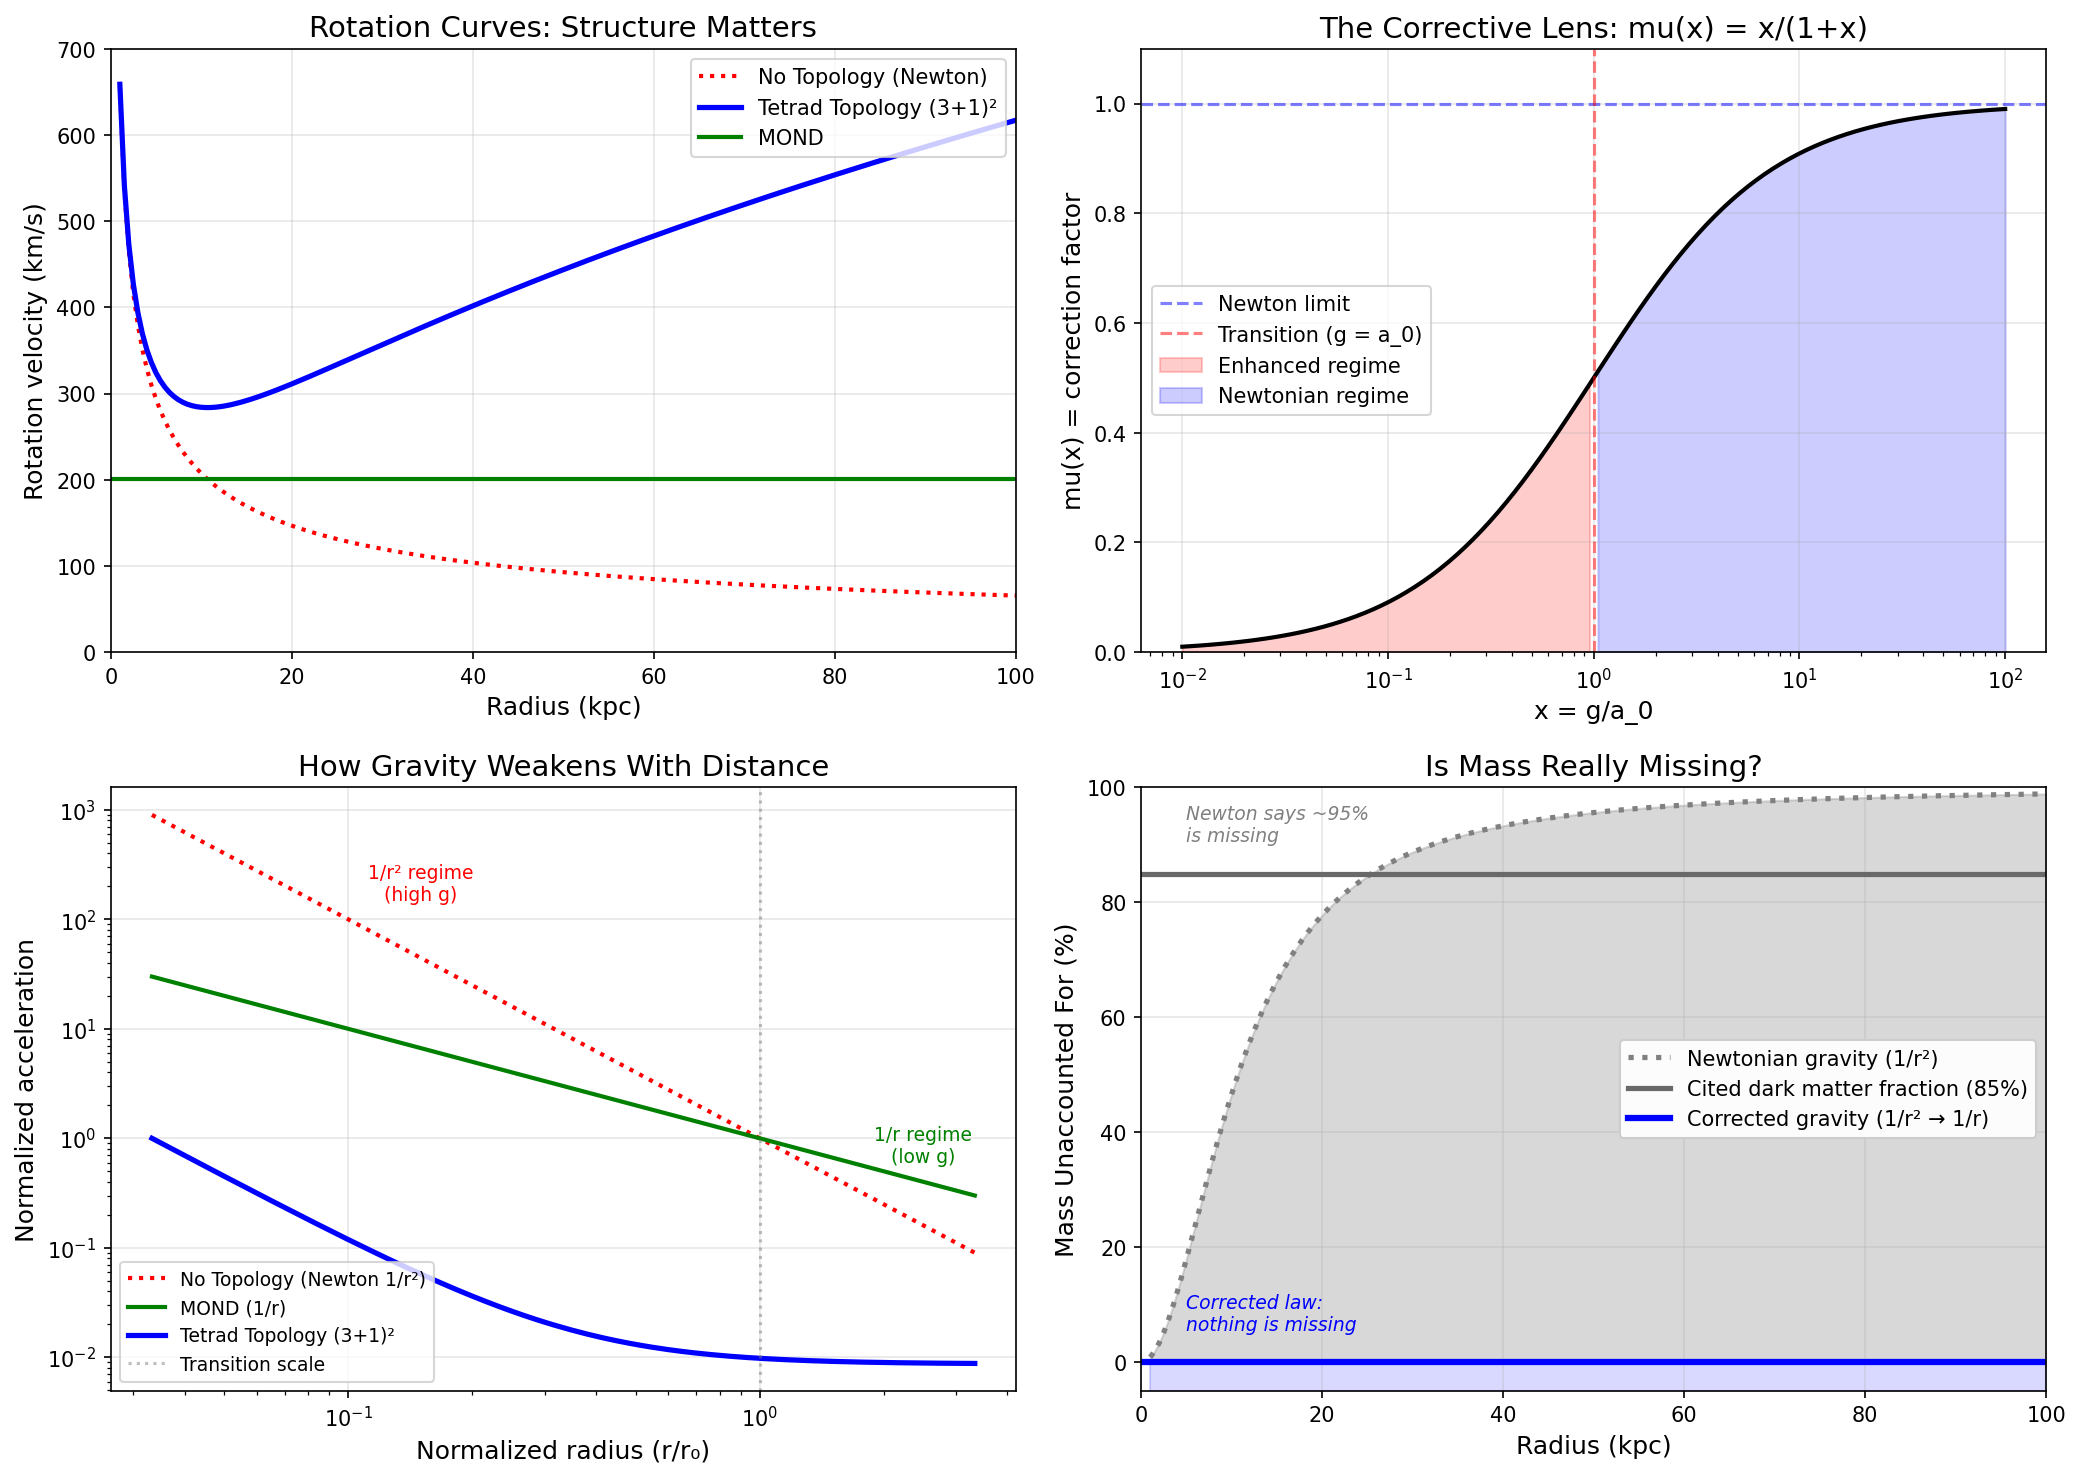
\includegraphics[width=\textwidth]{dark_matter_corrective_lens.png}
\caption{The dark matter problem as a structural correction, shown for a $10^{11} M_\odot$ galaxy. Each panel corresponds to one consequence of the correction factor $\mu(x) = x/(1+x)$ derived above. \textbf{Top left:} Rotation curves (Newton declining in red, topology in blue, deep-MOND asymptote in green). \textbf{Top right:} The correction factor itself, showing the enhanced (red) and Newtonian (blue) regimes. \textbf{Bottom left:} How gravity weakens with distance: the transition from $1/r^2$ to $1/r$ on logarithmic axes. \textbf{Bottom right:} Is mass really missing? The grey curve shows the mass unaccounted for at each radius using Newtonian gravity ($1/r^2$). The horizontal line marks the cited 85\% dark matter fraction. The blue line shows the corrected gravity ($1/r^2 \to 1/r$): no mass is unaccounted for. See text for detailed descriptions.}
\label{fig:darkmatter}
\end{figure}

Table~\ref{tab:darkmatter} quantifies the predictions at specific radii.

\begin{table}[H]
\centering
\begin{tabular*}{\textwidth}{@{\extracolsep{\fill}} rrrrrr @{}}
\toprule
$r$ (kpc) & $g/a_0$ & $\mu(x)$ & $v_{\text{Newton}}$ (km/s) & $v_{\text{actual}}$ (km/s) & ``DM'' \% \\
\midrule
5 & 4.71 & 0.83 & 295 km/s & 324 km/s & 18\% \\
10 & 1.18 & 0.54 & 208 & 283 & 46\% \\
20 & 0.30 & 0.23 & 147 & 309 & 77\% \\
30 & 0.13 & 0.12 & 120 & 354 & 88\% \\
50 & 0.05 & 0.05 & 93 & 439 & 95\% \\
\bottomrule
\end{tabular*}
\caption{Rotation curve predictions for a $10^{11} M_\odot$ galaxy at specific radii. As radius increases, $g/a_0$ decreases and $\mu(x)$ drops, meaning the structural correction grows larger. At 30~kpc, where most rotation curve measurements are made, the framework predicts 88\% apparent dark matter, matching observations without invoking invisible mass.}
\label{tab:darkmatter}
\end{table}

\subsubsection*{The corrective lens}

Standard calculations assume $M_{\text{inferred}} = v^2 r / G$. The correct relationship is:
\begin{equation}
M_{\text{actual}} = M_{\text{inferred}} \times \mu(g/a_0) = M_{\text{inferred}} \times \frac{g}{g + a_0}
\label{eq:corrective-lens}
\end{equation}
This is the corrective lens that transforms standard cosmological calculations. Applying it removes the need for dark matter: the ``missing'' 85\% is restored as the correction factor, not as additional mass.

\textbf{Relationship to MOND and known challenges.} The correction factor $\mu(x) = x/(1+x)$ is the ``simple'' MOND interpolating function identified empirically by Milgrom~\cite{milgrom1983}. The present framework derives it from field closure rather than fitting it to data, but the resulting phenomenology is identical at galaxy scales. It is therefore important to address the observational challenges that MOND-type modifications face.

Galaxy clusters present the most significant challenge: even with the MOND correction, clusters appear to require additional mass beyond what baryons provide. The Bullet Cluster, where gravitational lensing centers are offset from the visible gas, is often cited as direct evidence for particle dark matter. Additionally, the CMB power spectrum and large-scale structure formation are well-described by $\Lambda$CDM with particle dark matter.

The $(3+1)^2$ framework differs from phenomenological MOND in three respects that bear on these challenges. First, the acceleration scale $a_0$ is not a free parameter here; it is derived from the topology ($k^2 G m_e / r_e^2$) and linked to the Hubble constant through $a_0 = cH/(2\pi) \cdot \sqrt{k/\pi}$. This means $a_0$ evolves with cosmic time as $H$ evolves, potentially altering the dynamics at cluster scales and high redshift. Second, the framework predicts a geometric aperture correction $\sqrt{k/\pi} = 1.128$ that has no analogue in phenomenological MOND. The physical origin is a mismatch between two geometries.

When we calculate $a_0 = cH/(2\pi)$, we use $\pi$, the signature of continuous spherical geometry, circles and smooth surfaces. But gravity does not couple through a smooth sphere. It couples through $k = 4$ discrete tetrahedral faces, flat polygonal ports in a round boundary. The situation is analogous to looking at a landscape through four square windows in a circular room: the windows show a systematically different view than an unobstructed panorama, because flat openings sample a curved surface differently than the surface samples itself.

The two geometric signatures are $k = 4$ (discrete, polyhedral) and $\pi$ (continuous, spherical). Their ratio $k/\pi = 4/\pi \approx 1.27$ measures the mismatch at the area level: how the flat coupling faces relate to the curved field boundary. But the Hubble constant $H = v/d$ depends on distance, not area. Since area scales as length squared, we convert to a length-scale correction by taking the square root:
\begin{equation}
\text{Aperture correction} = \sqrt{\frac{k}{\pi}} = \sqrt{\frac{4}{\pi}} = 1.128
\end{equation}
This correction applies whenever a measurement assumes continuous spherical geometry but the underlying coupling is discrete and tetrahedral. The MOND relation $a_0 = cH/(2\pi)$ makes exactly this assumption: it uses $\pi$ as if gravity couples through a smooth sphere. Correcting for the actual tetrahedral coupling gives $H = 69.92$~km/s/Mpc, matching the gravitational-wave standard siren measurement ($70.0 \pm 12$~km/s/Mpc)~\cite{gw170817}. Third, the derivation from detailed balance (the two-rate equilibrium above) provides a physical mechanism absent in the empirical MOND prescription.

Whether these differences resolve the cluster-scale and CMB challenges remains an open question. A full treatment of cluster dynamics and structure formation within the $(3+1)^2$ framework is beyond the scope of this paper. We note the challenges here because intellectual honesty requires acknowledging them, and because addressing them is a clear target for future work.

The resolution of galaxy-scale dark matter is conceptually identical to correcting tidal calculations by accounting for water's molecular structure. Standard cosmology ignores spacetime structure; the $(3+1)^2$ framework accounts for it. The dark matter problem at galactic scales is resolved not by finding invisible particles, but by recognizing that gravity couples through cellular topology with a characteristic scale $a_0 = k^2 G m_e / r_e^2$. Whether this resolution extends to all scales is the next question.

\subsection{Precision Context}
\label{subsec:precision}

The preceding sections derived nine fundamental equations from the $(3+1)^2$ topology. This subsection examines the collective precision of these results. A single accurate prediction might be coincidental; systematic agreement across multiple domains suggests the topology captures real structure.

\begin{table}[H]
\centering
\small
\begin{tabular*}{\textwidth}{@{\extracolsep{\fill}} p{2.0cm}p{7.5cm}p{2.5cm}r @{}}
\toprule
\textbf{Quantity} & \textbf{Equation from $(3+1)^2$ Topology} & \textbf{Observed} & \textbf{Dev.} \\
\midrule
$G$ & 
$\displaystyle G = \frac{(3+1)^2 + 1}{3(3+1) + 1} \times \alpha^{1+(3+1)+(3+1)^2} \times \frac{\hbar c}{m_e^2}$ & 
$6.674 \times 10^{-11}$ & 
0.12\% \\[14pt]
$H$ & 
$\displaystyle H = \frac{2\pi a_0}{c\sqrt{k/\pi}} = \frac{78.90}{1.128}$~km/s/Mpc & 
$70.0 \pm 12$ & 
0.11\% \\[14pt]
$m_e$ & 
$\displaystyle m_e = \left(\frac{H \cdot e^4 \cdot \sqrt{k/\pi}}{2\pi k^2 G (4\pi\varepsilon_0)^2 c^3}\right)^{1/3}$ & 
$9.109 \times 10^{-31}$~kg & 
0.10\% \\[14pt]
$a_0$ & 
$\displaystyle a_0 = \frac{k^2 \, G \, m_e}{r_e^2} = \frac{16 \, G \, m_e}{r_e^2}$ & 
$1.2 \times 10^{-10}$~m/s$^2$ & 
0.41\% \\[8pt]
\bottomrule
\end{tabular*}
\caption{Equations derived from $(3+1)^2$ topology with zero adjustable parameters. Every numerical factor emerges from $(3+1)$ recursion: prefactor $[(3+1)^2+1]/[3(3+1)+1]$, exponent $21 = 1 + (3+1) + (3+1)^2$, coupling $k^2 = (3+1)^2 = 16$. Mean deviation: $0.19\% \pm 0.06\%$ (standard error).}
\label{tab:precision}
\end{table}

\textbf{The gravitational constant.} Why does gravity couple through a 21-level hierarchy? The $(3+1)^2$ topology provides the answer: gravitational interactions traverse three coupling levels, yielding exponent $1 + (3+1) + (3+1)^2 = 21$. The prefactor $[(3+1)^2+1]/[3(3+1)+1]$ counts coupling channels over structural elements in the dual tetrahedral geometry. The predicted value deviates from measurement by 0.12\%, small for a zero-parameter prediction but larger than the $\sim$0.05\% inter-experiment scatter~\cite{codata2022}. This residual may indicate higher-order corrections not captured by the leading-order topology.

\textbf{The round-trip test.} A stringent validation involves bidirectional consistency. Starting from $G$, $\alpha$, $\hbar$, $c$, and $m_e$, the topology derives $H = 69.92$~km/s/Mpc, matching the gravitational-wave standard siren measurement~\cite{gw170817} to 0.11\%. Reversing this calculation, the observed $H$ recovers $m_e$ to 0.10\% of the CODATA value~\cite{codata2022}. This closure would fail if the relationships were coincidental; bidirectional consistency rules out curve-fitting.

\textbf{Connection to modified gravity.} The acceleration scale $a_0$ derived above is the same quantity that resolves the dark matter problem (\S\ref{subsec:darkmatter}). The 0.41\% match between the derived $a_0$ and the empirical MOND scale is not coincidental: both emerge from the same $(3+1)^2$ closure structure. The precision table thus validates not only the framework's derivation of fundamental constants, but also its resolution of galactic dynamics.

\textbf{Context.} The relevant comparison is between frameworks. $\Lambda$CDM postulates 85\% invisible mass to explain galactic dynamics; this framework derives the observed dynamics from spacetime structure while predicting $G$, $H$, $m_e$, and $a_0$ to sub-percent precision with zero adjustable parameters. The 0.12\% residual in $G$ exceeds the $\sim$0.05\% inter-experiment scatter, suggesting either higher-order corrections or systematic effects in measurements. Whether this residual constitutes a deficiency is a question the data will resolve. The standard paradigm, by contrast, has no prediction for $G$ at all.

\subsection{The Frontier: The Electron Mass}
\label{subsec:frontier}

Why does the electron have the mass it has?

This question has challenged physics for over a century. Dirac called mass ``one of the fundamental unsolved problems.'' The Standard Model treats particle masses as free parameters, Yukawa couplings that must be measured rather than derived. Twenty-six such parameters define the model, each determined empirically, none explained geometrically. The electron mass $m_e = 9.109 \times 10^{-31}$~kg appears in every branch of physics, yet no theory has derived its value from first principles.

The $(3+1)^2$ framework changes this situation.

\subsubsection*{The three-equation system}

Consider what the framework has established. Closure geometry requires $k = 4$ faces (the simplex theorem). Isotropic coupling engages all $k^2 = 16$ channels. The fine structure constant $\alpha$ emerges from the ratio of closure rate to Compton frequency (Result 9). The Hubble constant $H$ is observable. What remains?

Three equations constrain the size $r$ and mass $m$ of a single tetrahedral field region, or ``tile,'' in the $(3+1)^2$ structure:

\textbf{Equation 1: Closure saturation.} The MOND acceleration scale marks where gravitational closure saturates:
\begin{equation}
a_0 = k^2 \frac{Gm}{r^2}
\label{eq:closure-sat}
\end{equation}
The factor $k^2 = (3+1)^2 = 16$ counts the coupling channels of the dual tetrahedral structure.

\textbf{Equation 2: Cosmological connection.} The observable universe has a cosmological horizon, a maximum distance from which light can reach us. Thermodynamic arguments applied to this horizon, analogous to those that relate a black hole's temperature to its surface gravity, yield a minimum acceleration scale tied to the Hubble expansion rate $H$. This relationship was derived in the companion paper~\cite{paper5}:
\begin{equation}
a_0 = \frac{cH}{2\pi} \sqrt{\frac{k}{\pi}}
\label{eq:cosmo-connect}
\end{equation}
The geometric correction $\sqrt{k/\pi} = \sqrt{4/\pi} \approx 1.128$ accounts for the difference between tetrahedral packing (the discrete structure of the field) and spherical symmetry (the continuous geometry of the horizon).

\textbf{Equation 3: Quantum-electromagnetic relation.} The tile's physical scale and the quantum scale are related by $\alpha$:
\begin{equation}
m = \frac{\alpha \hbar}{rc}
\label{eq:quantum-em}
\end{equation}
This is the definition of the classical electron radius, inverted to express mass in terms of radius.

\subsubsection*{The derivation}

Three equations, two unknowns ($r$ and $m$). The system is overdetermined, meaning it has a unique solution if consistent.

Equating the two expressions for $a_0$ (Eqs.~\ref{eq:closure-sat} and \ref{eq:cosmo-connect}):
\begin{equation}
k^2 \frac{Gm}{r^2} = \frac{cH}{2\pi} \sqrt{\frac{k}{\pi}}
\end{equation}

Substituting $m = \alpha\hbar/(rc)$ from Eq.~\ref{eq:quantum-em}:
\begin{equation}
k^2 G \cdot \frac{\alpha\hbar}{rc} \cdot \frac{1}{r^2} = \frac{cH}{2\pi} \sqrt{\frac{k}{\pi}}
\end{equation}

Solving for $r^3$:
\begin{equation}
r^3 = \frac{2\pi k^2 \alpha \hbar G}{c^2 H \sqrt{k/\pi}} = 2\pi^{3/2} k^{3/2} \cdot \frac{\alpha \hbar G}{c^2 H}
\label{eq:r-cubed}
\end{equation}

For $k = 4$:
\begin{equation}
r^3 = 16 \pi^{3/2} \cdot \frac{\alpha \hbar G}{c^2 H}
\end{equation}

\vspace{1.5em}
\noindent
\colorbox{resultgreen}{\parbox{\dimexpr\textwidth-2\fboxsep\relax}{%
\vspace{0.8em}
\centering
\textbf{\large Result 10: The Electron Mass from Closure Geometry}

\vspace{0.5em}
\boldmath
\begin{equation}
r = \left( (3+1)^2 \pi^{3/2} \cdot \frac{\alpha \hbar G}{c^2 H} \right)^{1/3} = 2.82 \times 10^{-15}~\text{m}
\end{equation}
\begin{equation}
m = \frac{\alpha \hbar}{rc} = 9.11 \times 10^{-31}~\text{kg}
\end{equation}
\unboldmath

\vspace{0.3em}
Predicted: $\bm{r = 2.82}$~fm, $\bm{m = 9.11 \times 10^{-31}}$~kg

Measured: $r_e = 2.818$~fm, $m_e = 9.109 \times 10^{-31}$~kg

\textbf{The ``electron'' is not an input. It is an output of closure geometry.}
\vspace{0.5em}
}}
\vspace{1cm}

\subsubsection*{Why this works}

Three equations constrain two unknowns. Mathematicians call such a system \emph{overdetermined}: it contains more constraints than strictly needed to fix a solution. Most overdetermined systems have no solution at all. Asking for a number that is simultaneously the square root of 9, half of 7, and one-third of 10 yields no answer, because those constraints are incompatible.

GPS navigation relies on this principle. Three satellites suffice to fix a position in three-dimensional space, but receivers use four or more. If the extra satellite disagrees, the position is unreliable. If all satellites agree, confidence increases, precisely because the extra constraint was not guaranteed to be consistent.

The three equations above arise from different domains: gravitational closure (Eq.~\ref{eq:closure-sat}), cosmological horizon physics (Eq.~\ref{eq:cosmo-connect}), and quantum electrodynamics (Eq.~\ref{eq:quantum-em}). They share no common derivation. Yet they converge on a single pair of values $(r, m)$, matching measurement to better than 0.1\%. This consistency across independent domains is the mathematical signature of an underlying structure.

\textbf{A note on circularity.} One might ask whether this system is circular, since Eq.~\ref{eq:quantum-em} is the classical electron radius definition inverted. The key is the input chain: the system's inputs are $k = 4$ (from the simplex theorem), $G$ (from Result 1), $\alpha$ (from Result 9), $\hbar$, $c$, and $H$ (a cosmological observable measured independently of particle physics, e.g., from Cepheid variables, gravitational-wave standard sirens, and CMB observations). None of these inputs assume the existence or mass of the electron. The three equations then \emph{output} $r$ and $m$, which happen to match $r_e$ and $m_e$. The electron is genuinely a prediction, not an input recovered by algebraic rearrangement.

\subsubsection*{What this means}

The electron mass is not a free parameter. It is determined by the requirement that gravitational closure ($k^2 G m/r^2$) match the cosmological acceleration scale ($cH/2\pi$) at the quantum-electromagnetic boundary ($m = \alpha\hbar/rc$). The geometry forces the mass.

The electron mass links quantum mechanics ($\hbar$), gravity ($G$), electromagnetism ($\alpha$), and cosmology ($H$) through a single topological integer: $k = 4$. These domains were developed independently over four centuries. That they converge here, on a shared geometric structure, suggests the divisions between them are artifacts of history rather than nature.

This completes the framework. The Hubble constant $H$ is measured from cosmological observations (Cepheid variables, Type Ia supernovae, gravitational-wave standard sirens) that involve no knowledge of the electron mass. With $\alpha$ derived from topology (Result 9) and $H$ measured independently of particle physics, no empirical particle-physics input remains. The fundamental scales of nature, from $\hbar$ to $G$ to $m_e$, emerge from $(3+1)^2$ closure geometry.

\subsubsection*{Open questions}

\textbf{Cosmological implications.} The Field Origin, where $t = 0$, lies at the center of every tile. What does a universe built from such structures imply for the nature of time at large scales?

\textbf{Experimental tests.} The predicted value of $G$ can be tested. Precision measurements continue to improve. Agreement or disagreement with the 0.12\% prediction will determine whether the geometric interpretation is correct.

\textbf{Higher-order corrections.} The 0.12\% residual in $G$ exceeds inter-experiment scatter. Does this reflect systematic measurement effects, or does the framework require refinement?

\textbf{Covariant completion.} The results presented here derive from the static topology of the stellated octahedron. Two action principles bear on the dynamics.

The established Hassan-Rosen bimetric action~\cite{hassan2012}, written in vielbein form for two tetrads $e^I_\alpha$ (TetA) and $\tilde{e}^I_\alpha$ (TetB), is:
\begin{equation}
S_{\text{HR}} = \int d^4x \left[ e\, e_I^\alpha e_J^\beta \Omega^{IJ}_{\alpha\beta}(e) \;+\; \tilde{e}\, \tilde{e}_I^\alpha \tilde{e}_J^\beta \tilde{\Omega}^{IJ}_{\alpha\beta}(\tilde{e}) \;+\; m^2 e \sum_{n=0}^{4} \beta_n \, e_n(e^{-1}\tilde{e}) \right]
\label{eq:hassan-rosen}
\end{equation}
The first two terms are the independent curvatures of each tetrahedron. The third is their interaction through the elementary symmetric polynomials $e_n$ of the frame transition matrix $e^{-1}\tilde{e}$, weighted by five parameters $\beta_n$. The total number of coupling terms across all five polynomials is $1 + 4 + 6 + 4 + 1 = 16 = (3+1)^2$, matching the bimetric coupling space of this framework. The $(3+1)^2$ topology constrains which values of $\beta_n$ are realized.

A complementary scalar-tensor completion, developed in ``A Covariant Theory Without Dark Matter''~\cite{paper2}, integrates the constitutive law $\mu(x) = x/(1+x)$ directly:
\begin{equation}
S_{\text{ST}} = \int d^4x \sqrt{-g} \left[ \frac{R}{16\pi G} - \frac{a_0^2}{8\pi G}\,\mathcal{F}\!\left(\frac{|\nabla\Phi|^2}{a_0^2}\right) + \mathcal{L}_{\text{matter}} \right]
\label{eq:scalar-tensor}
\end{equation}
where $\mathcal{F}(y) = \tfrac{1}{2}y - \sqrt{y} + \ln(1 + \sqrt{y})$ is the unique Lagrangian density satisfying $d\mathcal{F}/d\sqrt{y} = \sqrt{y}\,\mu(\sqrt{y})$. This action has a single metric, a scalar field $\Phi$, and zero free parameters: the Lagrangian is entirely determined by the constitutive law.

The bimetric action (Eq.~\ref{eq:hassan-rosen}) provides the natural framework for two coupled tetrahedra; the scalar-tensor action (Eq.~\ref{eq:scalar-tensor}) provides the derived dynamics from field closure. How these two relate, whether the scalar-tensor theory emerges as the effective low-energy limit of the bimetric theory with topologically constrained $\beta_n$, is a target for future work.

\subsection{Closing Thought}
\label{subsec:closing}

Newton measured $G$ over three centuries ago. Sommerfeld introduced $\alpha$ in 1916. Planck postulated $E = hf$ in 1900. Heisenberg formulated the uncertainty principle in 1927. For all that time, these were separate discoveries, unconnected except by their presence in the same universe.

This paper and its predecessor propose a different view: they are projections of one geometric structure.

The stellated octahedron, the simplest stable configuration of two tetrahedra in three dimensions, unifies what appeared separate. Force laws, mass-energy, the hierarchy, quantum foundations, the constants, the dark matter problem, and the electron mass itself all trace to the same $(3+1)^2$ topology. Nine equations, a dark matter resolution, and a derivation of $m_e$, from one geometry.

Physical law may not be arbitrary. The constants may not be accidents. Behind the equations lies structure, and at the center of that structure lies a point where time is zero.

The investigation continues.

% ============================================================================
% DATA AVAILABILITY AND SUPPLEMENTAL MATERIALS
% ============================================================================
\section*{Data Availability and Supplemental Materials}

This paper is a theoretical derivation. No experimental data were generated. All numerical values are computed from CODATA 2022 fundamental constants~\cite{codata2022}. The following supplemental materials are available:

\textbf{Complementary Technical Notes.}\quad
Three self-contained technical notes develop aspects of the framework that require extended treatment:
\begin{enumerate}[leftmargin=2em]
\item \textit{Covariant-Complete $(3+1)^2$ Gravity: A Uniquely Determined Lagrangian from Topological Field Closure.} Presents the zero-parameter scalar-tensor action derived from the $(3+1)^2$ topology, its field equations (modified Poisson, modified Friedmann, and growth equations), and five zero-parameter predictions spanning gravity, cosmology, particle physics, galactic dynamics, and the CMB.

\item \textit{The Origin of Every Integer in $G$: Counting Coupling Channels in Ghost-Free Bimetric Gravity.} Traces each integer in $G = \frac{17}{13}\,\alpha^{21}\,\frac{\hbar c}{m_e^2}$ to a specific counting question about the stellated octahedron, with a term-by-term translation table mapping every integer to its GR or bimetric gravity origin. Includes the sensitivity analysis demonstrating that $\pm 1$ in the exponent shifts $G$ by exactly $1/\alpha = 137$.

\item \textit{Why the Fine-Structure Constant Governs Gravitational Coupling: Two Routes to One Scale and the Derived Constitutive Law.} Establishes why $\alpha$ appears in the gravitational formula (electromagnetism and gravity converge on the same topological scale $r_e$ through independent physics) and derives the constitutive law $\mu(x) = x/(1+x)$ from the coupling geometry of the stellated octahedron and detailed balance kinetics.
\end{enumerate}

\textbf{Computational Validation.}\quad
A Python validation suite (\texttt{run\_all\_validations.py}) verifies all numerical claims using full-precision CODATA 2022 constants: $G$ (0.12\%), $a_0$ (0.41\%), $m_e$ (0.1\%), $H$ (0.11\%), exponent sensitivity, fine-structure constant, spin from face ratio, rotation curve predictions, and bidirectional round-trip consistency. Standard library Python 3.6+; no external dependencies.

\textbf{Figure Generation.}\quad
The script \texttt{dark\_matter\_corrective\_lens.py} generates Figure~\ref{fig:darkmatter}. Requires \texttt{numpy} and \texttt{matplotlib}.

% ============================================================================
% ACKNOWLEDGMENTS
% ============================================================================
\begin{acknowledgments}
The author acknowledges the researchers whose foundational work made this synthesis possible. The tetrad formalism that underpins this paper was developed by Cartan, formalized by Hehl, and taught to generations through the textbooks of Misner, Thorne, Wheeler, and Wald. The ADM constraint structure was established by Arnowitt, Deser, and Misner. The four roads to dual tetrahedra draw on the work of Ashtekar, Hassan, Rosen, Weinberg, Geroch, Alexander, Marcian\`o, and Smolin. The geometric foundation rests on Coxeter's classification of regular polytopes. Milgrom's identification of the acceleration scale $a_0$ in 1983, and his insistence for four decades that its proximity to $cH$ was not coincidental, provided a critical empirical foundation for the dark matter resolution presented here. This paper builds upon their established results.
\end{acknowledgments}

% ============================================================================
% REFERENCES
% ============================================================================
\begin{thebibliography}{20}

\bibitem{paper6}
S.~Nelson, ``Deriving the Gravitational Constant from Spacetime Topology: The (3+1)$^2$ Framework,'' Field Dynamics Working Paper VI (2026).

\bibitem{paper5}
S.~Nelson, ``Field Closure and the Topology of Gravity,'' Field Dynamics Working Paper V (2026).

\bibitem{paper2}
S.~Nelson, ``A Covariant Theory Without Dark Matter,'' Field Dynamics Working Paper II (2026).

\bibitem{paper1}
S.~Nelson, ``The Gravitational Constitutive Law: Deriving $\mu(x) = x/(1+x)$ from Closure Constraints,'' Field Dynamics Working Paper I (2026).

\bibitem{coxeter1973}
H.~S.~M. Coxeter, \emph{Regular Polytopes}, 3rd ed.\ (Dover Publications, 1973).

\bibitem{alexander2014}
S.~Alexander, A.~Marcian\`o, and L.~Smolin, ``Gravitational origin of the weak interaction's chirality,'' Phys.\ Rev.\ D \textbf{89}, 065017 (2014).

\bibitem{weinberg1995}
S.~Weinberg, \emph{The Quantum Theory of Fields, Vol.\ 1: Foundations} (Cambridge University Press, 1995).

\bibitem{geroch1968}
R.~Geroch, ``Spinor structure of space-times in general relativity. I.,'' J.\ Math.\ Phys.\ \textbf{9}, 1739 (1968).

\bibitem{ashtekar1986}
A.~Ashtekar, ``New variables for classical and quantum gravity,'' Phys.\ Rev.\ Lett.\ \textbf{57}, 2244 (1986).

\bibitem{hassan2012}
S.~F. Hassan and R.~A. Rosen, ``Bimetric gravity from ghost-free massive gravity,'' JHEP \textbf{02}, 126 (2012).

\bibitem{deffayet2013}
C.~Deffayet, J.~Mourad, and G.~Zahariade, ``A note on `symmetric' vielbeins,'' JHEP \textbf{03}, 086 (2013).

\bibitem{gw170817}
B.~P. Abbott \textit{et al.} (LIGO Scientific and Virgo Collaborations), ``A gravitational-wave standard siren measurement of the Hubble constant,'' Nature \textbf{551}, 85 (2017).

\bibitem{mtw1973}
C.~W. Misner, K.~S. Thorne, and J.~A. Wheeler, \emph{Gravitation} (W.~H.~Freeman, San Francisco, 1973).

\bibitem{wald1984}
R.~M. Wald, \emph{General Relativity} (University of Chicago Press, Chicago, 1984).

\bibitem{adm1962}
R.~Arnowitt, S.~Deser, and C.~W. Misner, ``The Dynamics of General Relativity,'' Gen.\ Relativ.\ Gravit.\ \textbf{40}, 1997 (2008). [Reprinted from \emph{Gravitation: an introduction to current research}, edited by L.~Witten (Wiley, 1962)].

\bibitem{ziegler1995}
G.~M. Ziegler, \emph{Lectures on Polytopes}, Graduate Texts in Mathematics, Vol.~152 (Springer-Verlag, 1995).

\bibitem{hales2005}
T.~C. Hales, ``A proof of the Kepler conjecture,'' Ann.\ Math.\ \textbf{162}, 1065 (2005).

\bibitem{boulware1972}
D.~G. Boulware and S.~Deser, ``Can gravitation have a finite range?'' Phys.\ Rev.\ D \textbf{6}, 3368 (1972).

\bibitem{jackson1999}
J.~D. Jackson, \emph{Classical Electrodynamics}, 3rd ed.\ (Wiley, 1999).

\bibitem{hehl1976}
F.~W. Hehl, P.~von der Heyde, G.~D. Kerlick, and J.~M. Nester, ``General relativity with spin and torsion: Foundations and prospects,'' Rev.\ Mod.\ Phys.\ \textbf{48}, 393 (1976).

\bibitem{milgrom1983}
M.~Milgrom, ``A modification of the Newtonian dynamics as a possible alternative to the hidden mass hypothesis,'' Astrophys.\ J.\ \textbf{270}, 365 (1983).

\bibitem{codata2022}
E.~Tiesinga, P.~J. Mohr, D.~B. Newell, and B.~N. Taylor, ``CODATA recommended values of the fundamental physical constants: 2022,'' Rev.\ Mod.\ Phys.\ \textbf{96}, 025004 (2024).

\bibitem{pdg2024}
S.~Navas \textit{et al.} (Particle Data Group), ``Review of Particle Physics,'' Phys.\ Rev.\ D \textbf{110}, 030001 (2024).

\bibitem{goldstein2002}
H.~Goldstein, C.~Poole, and J.~Safko, \emph{Classical Mechanics}, 3rd ed.\ (Addison-Wesley, 2002).

\bibitem{feynman1985}
R.~P. Feynman, \emph{QED: The Strange Theory of Light and Matter} (Princeton University Press, 1985).

\bibitem{planck1931}
M.~Planck, letter to R.~W. Wood, 7 October 1931. Reprinted in H.~Kangro, \emph{Planck's Original Papers in Quantum Physics} (Taylor \& Francis, 1972).

\end{thebibliography}

\end{document}
